\chapter{Results and discussion}\label{chap:Results&Disc}
\section{PFCA sorption}
\subsection{Biochar-water sorption isotherms}
\cref{fig:sorption_isotherms} shows the sorption isotherms for PFPeA, PFHxA, PFHpA, PFOA, PFNA and PFDA on CWC, ULS and DSL biochars. The points generated from the batch tests were fitted using the Freundlich model (\cref{eq:FreundlichLinear}). For all compounds, the sorption isotherm for ULS was visibly higher than DSL, followed by CWC. The Freundlich sorption coefficients ($\log~K_F$), linearity coefficients ($n_F$), and correlation coefficients ($r^2$) are presented in \cref{tab:summary_stats_single}. Somewhat unexpectedly, sorption is strongest for the two sludge chars. Possible mechanisms for the strong sorption will be discussed in this section. Due to the fact that the research on sorption of PFAS to sewage sludge biochars presented in this thesis is novel, there is not, to the author's knowledge, currently available literature partitioning coefficients for PFAS to other sewage sludge biochars. However, comparisons can be made between the $\log~K_F$s found in this thesis, and commercially-produced activated carbons (AC) reported in previous studies. Sorption coefficients in this study (5.12-5.73) are equivalent to, or higher than, values for $\log~K_F$ of PFOA to AC found in other literature: 5.60 \citep{kupryianchyk2016biochar}, 4.45 \citep{hansen2010sorption}, and 4.74-5.42 \citep{silvani2019can}. 

\begin{figure}[tb]
    \centering
    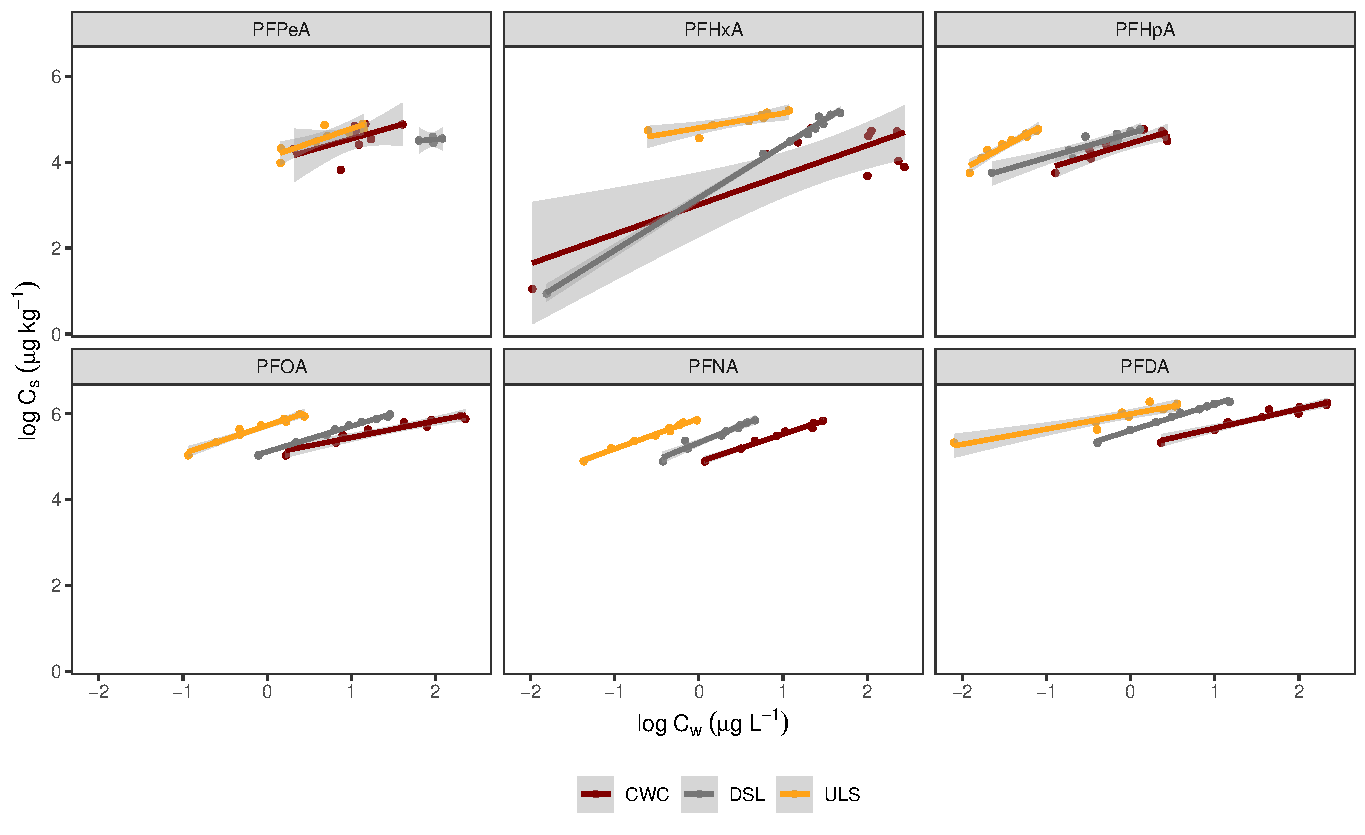
\includegraphics[width=\textwidth]{R/figs/Sorption_isotherms_single_BC.pdf}
    \caption{Freundlich sorption isotherms for PFPeA, PFHxA, PFHpA, PFOA, PFNA and PFDA in batch tests with three different biochars. Lines are obtained by linear regression.}
    \label{fig:sorption_isotherms}
\end{figure}

\begin{table}
\caption{Freundlich sorption parameters of single-compound isotherms in CWC, ULS and DSL (n=9). The error is presented as standard error. All $K_F$ data are in units of $\mathrm{(\mu g/kg)/(\mu g/L)^{n_F}}$.}
\centering
\adjustbox{max width=\textwidth}{%
\begin{threeparttable}
\label{tab:summary_stats_single}
\begin{tabular}{lllllllllllll} \toprule
PFCA & \multicolumn{4}{c}{ULS} & \multicolumn{4}{c}{DSL} & \multicolumn{4}{c}{CWC} \\ \cmidrule(l){2-5} \cmidrule(l){6-9} \cmidrule(l){10-13}
 & $\log~K_{F,BC}$ & $n_{F,BC}$ & $r^2$ & $p$ & $\log~K_{F,BC}$ & $n_{F,BC}$ & $r^2$ & $p$ & $\log~K_{F,BC}$ & $n_{F,BC}$ & $r^2$ & $p$ \\ \midrule
PFPeA & 4.10 ± 0.13 & 0.67 ± 0.16 & 0.74 & ** &  &  &  & $>$0.05 &  &  &  & $>$0.05 \\
PFHxA & 4.80 ± 0.06 & 0.34 ± 0.09 & 0.72 & ** & 3.30 ± 0.15 & 1.11 ± 0.11 & 0.93 & *** &  &  & & $>$0.05 \\
PFHpA & 5.98 ± 0.17 & 1.08 ± 0.11 & 0.93 & *** & 4.67 ± 0.06 & 0.57 ± 0.09 & 0.86 & *** & 4.44 ± 0.05 & 0.59 ± 0.11 & 0.80 & ** \\
PFOA & 5.73 ± 0.02 & 0.65 ± 0.05 & 0.95 & *** & 5.12 ± 0.02 & 0.60 ± 0.02 & 0.99 & *** & 5.06 ± 0.08 & 0.39 ± 0.05 & 0.90 & *** \\
PFNA & 5.89 ± 0.02 & 0.71 ± 0.03 & 0.99 & *** & 5.33 ± 0.03 & 0.80 ± 0.07 & 0.94 & *** & 4.88 ± 0.04 & 0.65 ± 0.04 & 0.98 & *** \\
PFDA & 6.00 ± 0.04 & 0.35 ± 0.05 & 0.86 & *** & 5.61 ± 0.02 & 0.61 ± 0.02 & 0.99 & *** & 5.22 ± 0.07 & 0.45 ± 0.04 & 0.94 & *** \\ \bottomrule
\end{tabular}
\begin{tablenotes}
\item Significance codes: *** $<$ 0.001, ** $<$ 0.01
\item Insignificant regressions (p $<$ 0.05) have been removed
\end{tablenotes}
\end{threeparttable}}
\end{table}

\subsection{Effect of PFCA chain length}
\begin{landscape}


\begin{figure}[tb]
    \centering
    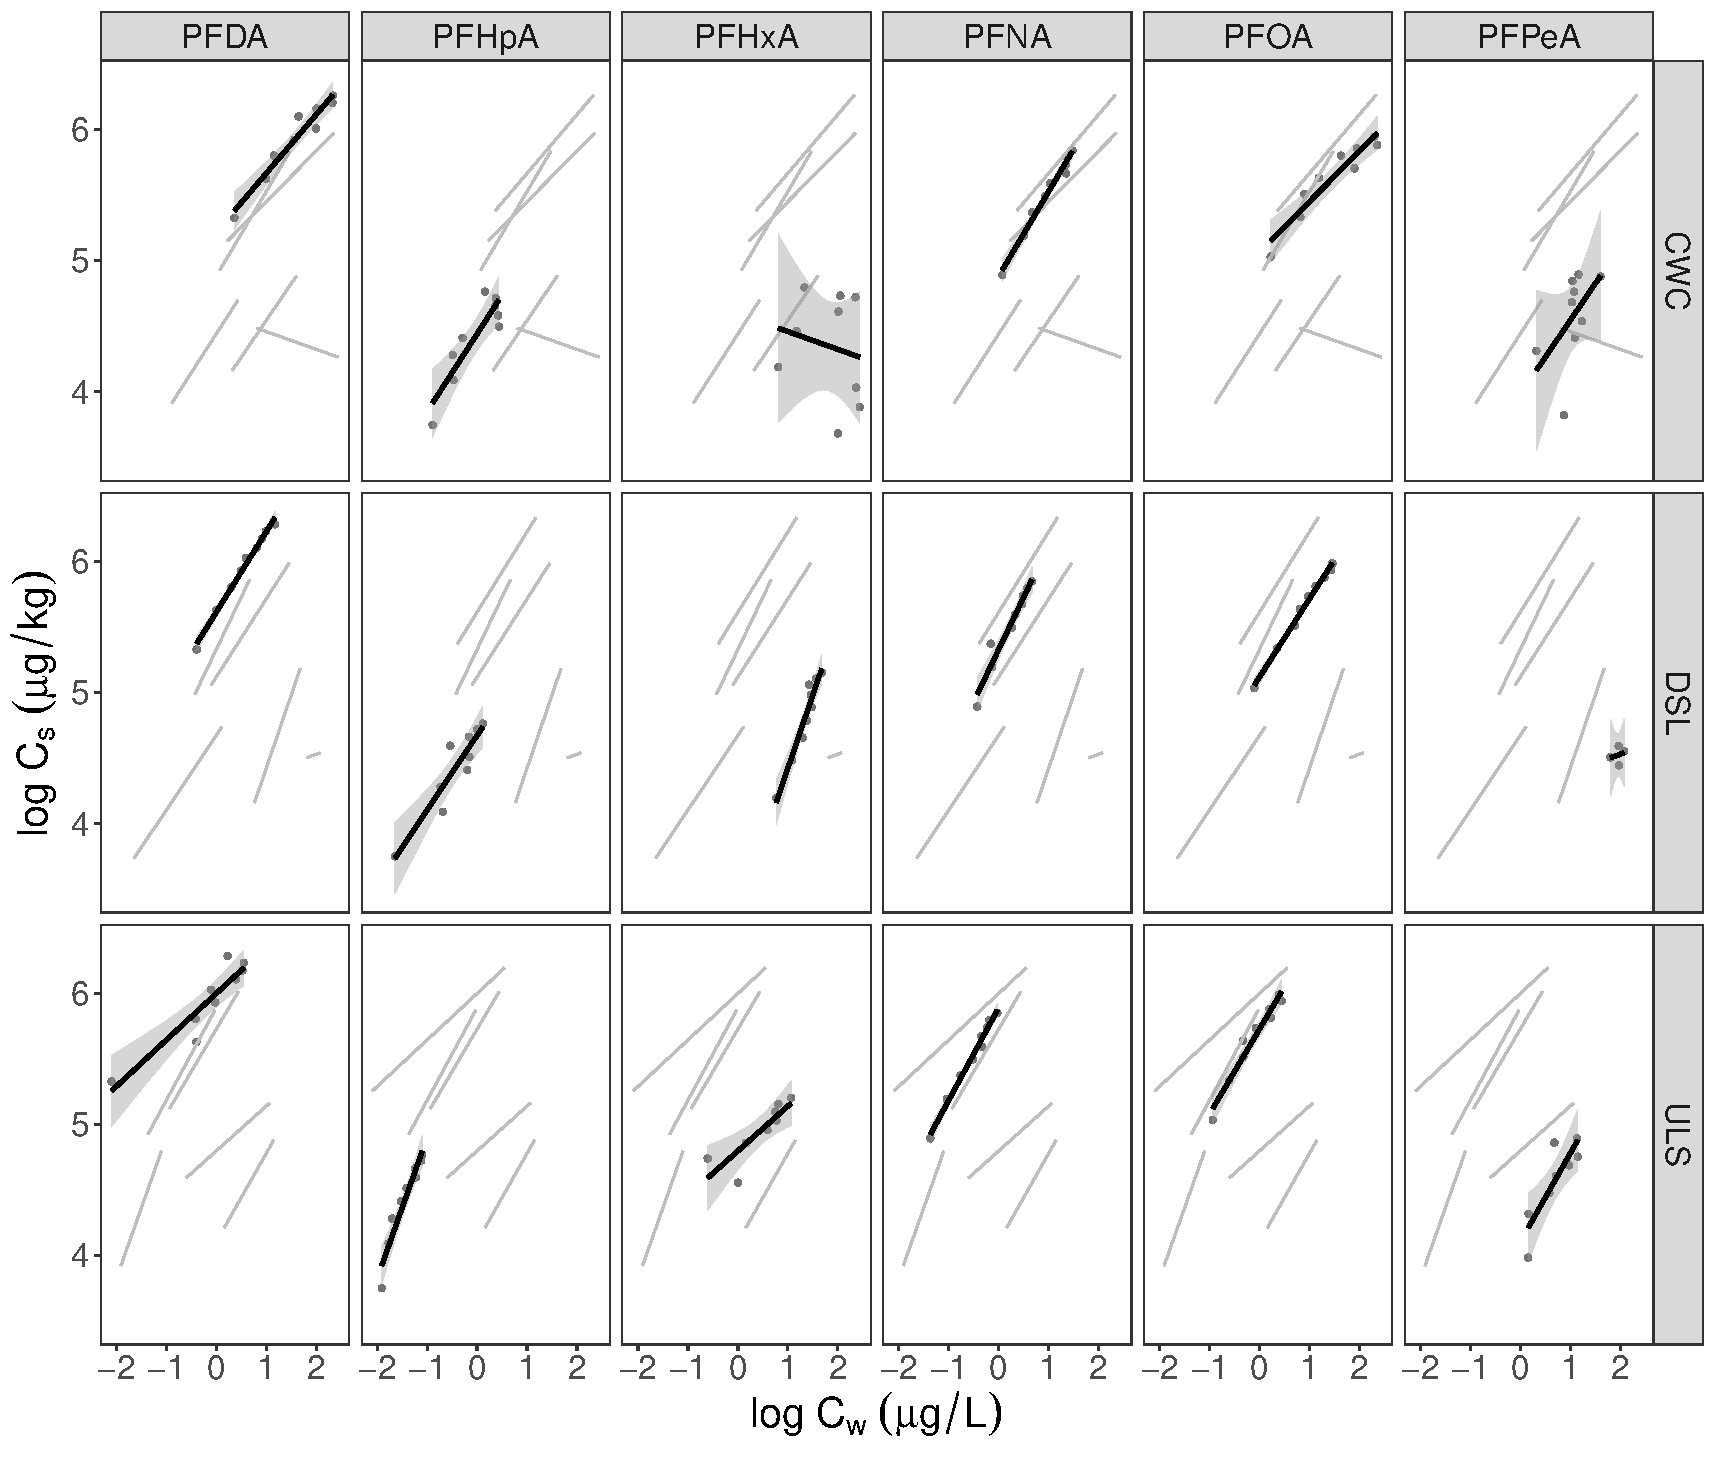
\includegraphics[height=0.8\textheight]{R/figs/BC_facet_isotherm.pdf}
    \caption{Single-compound Freundlich sorption isotherms for PFPeA, PFHxA, PFHpA, PFOA, PFNA and PFDA. Lines are obtained by linear regression. For comparison across chain length, the shaded gray lines are the isotherms from the other compounds with the same sorbent.}
    \label{fig:sorption_isotherms_all}
\end{figure}

\end{landscape} 
\subsubsection{PFCA chain length}
\Cref{fig:sorption_isotherms_all} shows sorption isotherms for the single-compound batch tests for CWC, ULS and DSL. The Freundlich coefficients ($\log~K_F$) reported are in units of $\mathrm{(\mu g/kg)/(\mu g/L)^{n_F}}$. Sorption to ULS increased in the order: PFPeA (CF4) $<$ PFHxA (CF5) $<$ PFOA (CF7) $<$ PFHpA (CF6) $<$ PFNA (CF8) $<$ PFDA (CF9) where $\log~K_F$ ranged from 4.10$\pm$0.13 to 6.00$\pm$0.04 . Sorption to DSL increased in the order: PFHxA (CF5) $<$ $<$ PFHpA (CF6) $<$ PFOA (CF7) $<$ PFNA (CF8) $<$ PFDA (CF9) where $\log~K_F$ ranged from 3.30$\pm$0.15 to 5.61$\pm$0.02. Sorption to CWC increased in the order: PFPeA (CF4) $<$ PFHpA (CF6) $<$ PFHxA (CF5) $<$ PFNA (CF8) $<$ PFOA (CF7) $<$ PFDA (CF9) where $\log~K_F$ ranged from $\log~K_F$ 3.98$\pm$0.36 to 5.22$\pm$0.07. Insignificant ($p>0.05$) isotherms have not been reported. Poor correlations for the isotherm regressions were achieved for the short-chain PFCAs (PFPeA, PFHxA, and PFHpA) when sorption isotherms were derived which can be attributed to poor sorption affinity to biochar. All Freundlich coefficients are listed in \cref{tab:summary_stats_single}. 

The sorption of PFAS increased with greater fluorinated chain length. A statistically significant relationship between $\log~K_F$ and CF\textsubscript{2} chain length was found for all three biochars (p$<$0.05) to PFOA, PFNA, and PFDA (\cref{fig:chainlength}) in accordance with previous studies \citep{Sorengard2019, fabregat2022examining, ahmed2020per}. There was a difference of 1.2-1.9 $\log~K_F$ units between the longest and the shortest PFCA chain (PFDA and PFPeA). This relationship suggests that hydrophobic interactions play a major role in sorption. For every CF\textsubscript{2} moiety, hydrophobic interactions between condensed aromatic structures in the biochar matrix increases, contributing to stronger sorption. Several mechanisms can explain why perfluorinated carboxylic acids increase in hydrophobicity with increasing chain length: 1) Due to a high molecular surface of the perfluorinated tail, a high cavity formation energy is needed to dissolve the compounds in water \citep{Arp2006}. For this reason, the compounds tend to be pushed water-solid interfaces, such as a biochar surface. Therefore, dissolution becomes increasingly energetically demanding with increasing chain length \citep{sigmund2022sorption}. 2) The perfluorinated chain is capable of the lowest van der Waals dispersive forces per molecular surface area compared to a hydrocarbon chain \citep{du2014adsorption}. The result is that PFAS has a much weaker attraction than hydrophobic organic compounds to water molecules when in the water cavity. For this reason, PFAS are both oil- and water repellent.  Generally, water cavity formation energy and van der Waals interactions have been considered insignificant for sorption of short-chain PFAS to solid phases (\textless C6) \citep{du2014adsorption}. They are, however, significant for long-chained PFCs (\textgreater C6) \citep{du2014adsorption} which corresponds with the chain length dependency found in this study.

\begin{figure}[tbh]
    \centering
    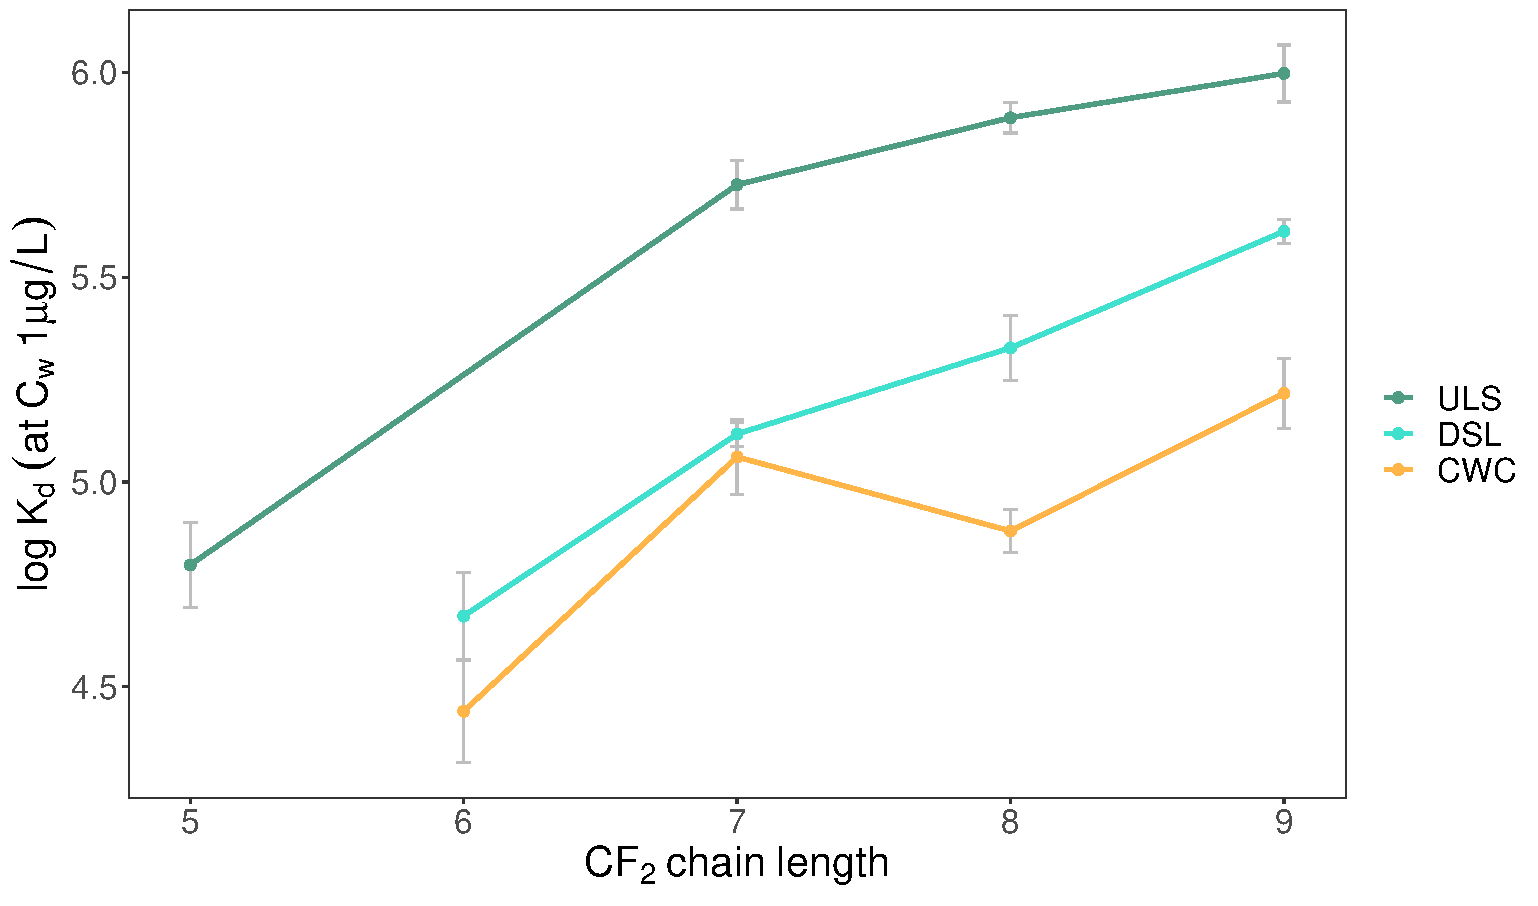
\includegraphics[width=0.7\textwidth]{R/figs/chain_length_Kd1ugL_plot.pdf}
    \caption{Relationship between $\log~K_F$ and chain length. Linear regression coefficients for ULS: $r^2$ = 0.92, $p$ = 0.04, DSL: $r^2$ = 0.98, $p$ = 0.01, CWC: $r^2$ = 0.68, $p$ = 0.17. Error bars are the propagated error of $\log~K_F$ and $n_F$.}
    \label{fig:chainlength}
\end{figure}

\subsubsection{PFAS functional groups} 
With the chain-length dependency on PFCA sorption found in this study (\cref{fig:chainlength}), electrostatic interactions by the negatively charged carboxylate functional group seems to be of secondary importance. However, especially for short-chain PFAS, the effect of the charge-assisted polar head cannot be disregarded. PFAS can engage simultaneously in hydrophobic interactions (perfluorinated chain) and electrostatic interactions (attraction and repulsion) with surface functional groups or dissolved ions (head) \citep{zhang2013sorption,sigmund2022sorption}. The different electrostatic interactions (cation bridging, biochar surface attraction and repulsion) are discussed more in depth in \cref{sec:inorganic}.

\cite{zhang2021sorption} found that sorption increased in the order PFBA $<$ PFBS $<$ PFOA $<$ PFOS for granular activated carbon and softwood-derived biochar. The difference between the PFSA and PFCA groups is that PFSAs have one more perfluorinated carbon than PFCAs, which has its terminal carbon bonded as a carboxylate (COO\textsuperscript{-}) instead. If one compares PFHpS to PFOA, which have the same number of $\mathrm{CF_2}$ moieties, the perfluorinated sulfonic acid still sorbs better. Researchers attribute this to: 1) A difference in molecular size because the sulfonate moiety is slightly larger than the carboxylate moiety. This results in a greater cavity formation energy for PFSAs. Hence, in water saturated conditions, the functional group is pushed towards water extremities \citep{yin2022insights,sigmund2022sorption}. In batch shaking experiments, this would be the biochar surfaces or artifacts. 2) Sulfonic acid is a stronger acid than carboxylic acid. This results in a stronger ionic interaction to positive charges of mineral phases in biochar ash \citep{arvaniti2015review}. 

%%%%%%%%%%%%%%%%%%%%%%%%%%%%%%%%%%%%%%%%%%%%%%%%%%%%%%%%%%%%%%%%%%%%%%%%%%%%%%%%%%%%%%%%%%%%%%%%%%%%%%%%%%%%%%%%%%%%%%%%%%%%%%%%%%%%%%%%%%%%%%%%%%%%%%%%%%%%%%%%%%%%%%%%%%%%%%%%%%%%%%%%%%%%%%%%%%%%%%%%%%%%%%%%%%%%%%%%%%%%%%%%%%%%%%%%%%%%%%%%%%%%%%%%%%%%%%%%%%%%%%%%%%%%%%%%%%%%%%%%%%%%%%%%%%%%%%%%%%%%%%%%%%%%%%%%%%%%%%%%%%%%%%%%%%%%%%%%%%%%%%%%%%%%%%%%%%%%%%%%%%%%%%%%%%%%%%%%%%%%%%%%%%%%%%%%%%%%%%%%%%%%%%%%%%%%%%%%%%%%%%%%%%%%%%%%%%%%%%%%%%%%%%%%%%%%%%%%%%%%%%%%%%%%%%%%%%%%%%%%%%%%%%%%%%%%%%%%%%%%%%%%%%%%%%%%%%%%%%%%%%%%%%%%%%%%%%%%%%%%%%%%

\section{The effect of biochar properties on sorption}
This section relates the distribution coefficients derived for ULS, DSL and CWC biochars to the following BC characteristics: main elements (C, H, O, N), trace elements (Ca and Fe), surface area (\acrshort{SA}), and pore volume (\acrshort{PV}) in an attempt to gain insight into possible sorption mechanisms. In the comparison between sorbent properties and sorption coefficients for each biochar feedstock, PFOA, PFNA and PFDA have been used because they exhibited the best sorption isotherms. The Freundlich coefficients ($\log~K_F$) have been normalized to 1 $\mu g~L^{-1}$ which is used as the distribution coefficient ($K_d$) in this discussion. Conducting multivariate analyses between biochar $K_d$ and the different supporting parameters for the biochar samples were desired but not statistically valid due to no degrees of freedom with only 3 samples. Therefore, the discussion on the effects of biochar properties on sorption will be limited to discerning trends with SA, PV, C, Ca and Fe. 

\subsection{Surface area and pore volume}\label{sec:SAPV}

\begin{table}
\centering
\caption{Surface area (SA), pore volume (PV), elemental content (C, O, H, N) and ratios for the biochars produced for the batch tests.}
\adjustbox{max width=\textwidth}{
\label{tab:SAPV}
\begin{tabular}{lcccccccccccc}
\toprule
Biochar & \multicolumn{3}{l}{N\textsubscript{2} sorption} & \multicolumn{2}{l}{CO\textsubscript{2} sorption} & \multicolumn{4}{l}{Elemental content} & \multicolumn{3}{c}{Element ratio} \\
sorbent & \multicolumn{3}{l}{(pores \textgreater 1.5 nm)} & \multicolumn{2}{l}{(pores 0.4-1.5 nm)} & & & & & & \\ \cmidrule(l){2-4} \cmidrule(l){5-6} \cmidrule(l){7-10} \cmidrule(l){11-13} 
& BET SA  & BJH PV  & DFT SA & DFT PV & C & O & H & N & O/C & H/C & N/C \\
& ($\mathrm{m^2~g^{-1}}$) & (cm\textsuperscript{3} g\textsuperscript{-1}) & ($\mathrm{m^2~g^{-1}}$) & (cm\textsuperscript{3} g\textsuperscript{-1}) & (\%) & (\%) & (\%) & (\%) & & & \\ \midrule
CWC & 323 & 0.017 & 683 & 0.186 & 91.4 & 5.50 & 1.01 & 0.69 & 0.06 & 0.01 & 0.008 \\
ULS & 128 & 0.126 & 165 & 0.047 & 29.6 & 57.1 & 1.24 & 1.13 & 1.9  & 0.04 & 0.04 \\
DSL & 110 & 0.111 & 87  & 0.027 & 13.5 & 61.4 & 1.05 & 0.82 & 4.6  & 0.08 & 0.06 \\ \bottomrule
\end{tabular}}
\end{table}

\subsubsection{Pore size distribution between 0.4-1.5 nm}
\cref{tab:SAPV} shows the total surface area (SA, m\textsuperscript{2}/g) and pore volume (PV, cm\textsuperscript{3}/g) for the three biochars used in the sorption experiments in this study. SA of CWC biochar (683 m\textsuperscript{2} g\textsuperscript{-1}) was $\sim$six times higher than that of ULS and DSL biochars (165 and 87  m\textsuperscript{2} g\textsuperscript{-1}, respectively), and PV also reflected the same order. Previous research has postulated that large internal surface areas and pore volumes are desirable for strong sorption of organic contaminants because they increase the fraction of active sorption sites \citep{ahmed2020per,Hale2016}. The high SA and PV of CWC suggest that this biochar has the highest fraction of active sites compared to ULS and DSL within the micropore range ($\le$ 2 nm). However, the pore size distribution (PSD) in terms of SA and PV of pores available for CO\textsubscript{2} adsorption (0.4-1.5 nm) shown in \cref{fig:PZD_small} shows that nearly 80\% of the SA and 60\% of the PV of CWC are located in pores smaller than 0.6 nm. These are referred to as ultra micropores \citep{bardestani2019experimental}. To find out whether PFCAs can be accommodated in these ultra micropores, \cref{tab:molecsize} lists effective cross-sectional diameter ($D_{eff}$) and maximum diameter ($D_{max}$) of each PFCA (the definitions of $D_{eff}$ and $D_{max}$ are illustrated in \cref{fig:molecularSize}). PFCAs C5-C10 range from 0.45-0.72 nm ($D_{eff}$) to 0.96-1.54 nm ($D_{max}$). Since the respective perfluorinated chains are too large and rigid to enter, most pores ($<$ 0.6 nm) turned out to be inaccessible to the PFCA molecules \citep{yu2009sorption}. Additionally, pores that are too small make it difficult for the compounds to adjust their shape to the pore walls in order to be able to come close enough to sorb to the pore wall surface. For this reason, they may get stuck in a cross-sectional position that blocks the pores for diffusion of new sorbates. 

Maximum sorption is achieved when the molecular dimensions of PFAS match the pore size and shape of the sorbent \citep{Hale2016}. Since the \acrshort{PSD} within the CO\textsubscript{2}-range is dominated by ultra micropores, sorption of PFPeA, PFHxA, and PFHpA is only possible if the congeners enter the pores at the exact right angle. PFOA, PFNA, and PFDA will experience size exclusion because the molecular size is too large in any direction (\cref{tab:molecsize}). In addition, these pores are easily blocked. This means that sorption of PFAS in the CO\textsubscript{2}-range is insignificant and cannot explain the differences in the $\log~K_F$ obtained for the biochar feedstocks, especially since strongest sorption was measured for long-chain PFCAs.

\begin{figure}[htb]
    \centering
    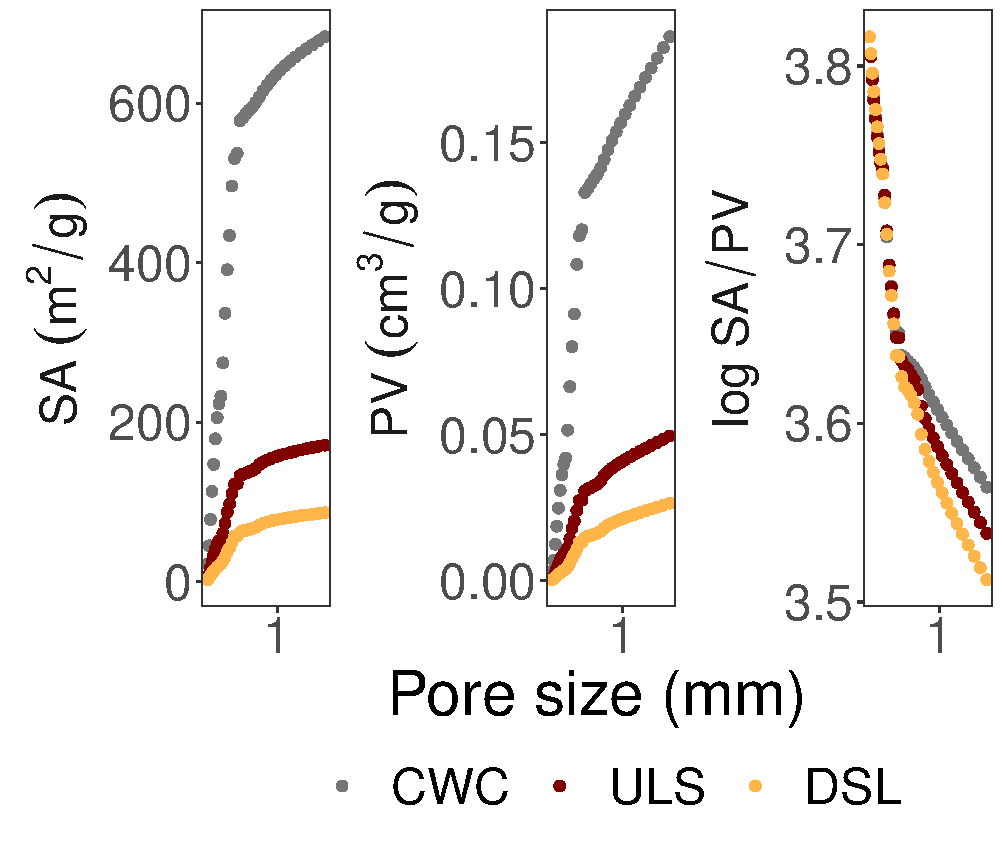
\includegraphics[width=\textwidth]{R/figs/PZD_SAPV_C_small_plot.pdf}
    \caption{Cumulative pore size distribution for pores 0.4-1.5 nm using DFT.}
    \label{fig:PZD_small}
\end{figure}

\begin{table}
\caption{Effective cross-sectional diameter ($D_{eff}$) and maximum diameter ($D_{max}$) of TCs interpolated and extrapolated by linear regression from calculations performed by \cite{inoue2012size} on PFOA and other PFCAs with chain lengths 11-18.}
\centering
\begin{threeparttable}
\label{tab:molecsize}
\begin{tabular}{lcrr}
\toprule
Compound & Chain & $D_{eff}$ & $D_{max}$ \\ 
& length & (nm) & (nm) \\ \midrule
PFPeA & 5  & 0.45  & 0.96  \\
PFHxA & 6  & 0.50  & 1.08  \\
PFHpA & 7  & 0.56  & 1.19  \\
PFOA\textsuperscript{*} & 8 & 0.61 & 1.36 \\
PFNA & 9 & 0.67 & 1.42  \\
PFDA & 10 & 0.72 & 1.54  \\ \bottomrule                                    
\end{tabular}
\begin{tablenotes}
\item \textsuperscript{*} Value from \cite{inoue2012size}
\end{tablenotes}
\end{threeparttable}
\end{table}

\begin{figure}
    \centering
    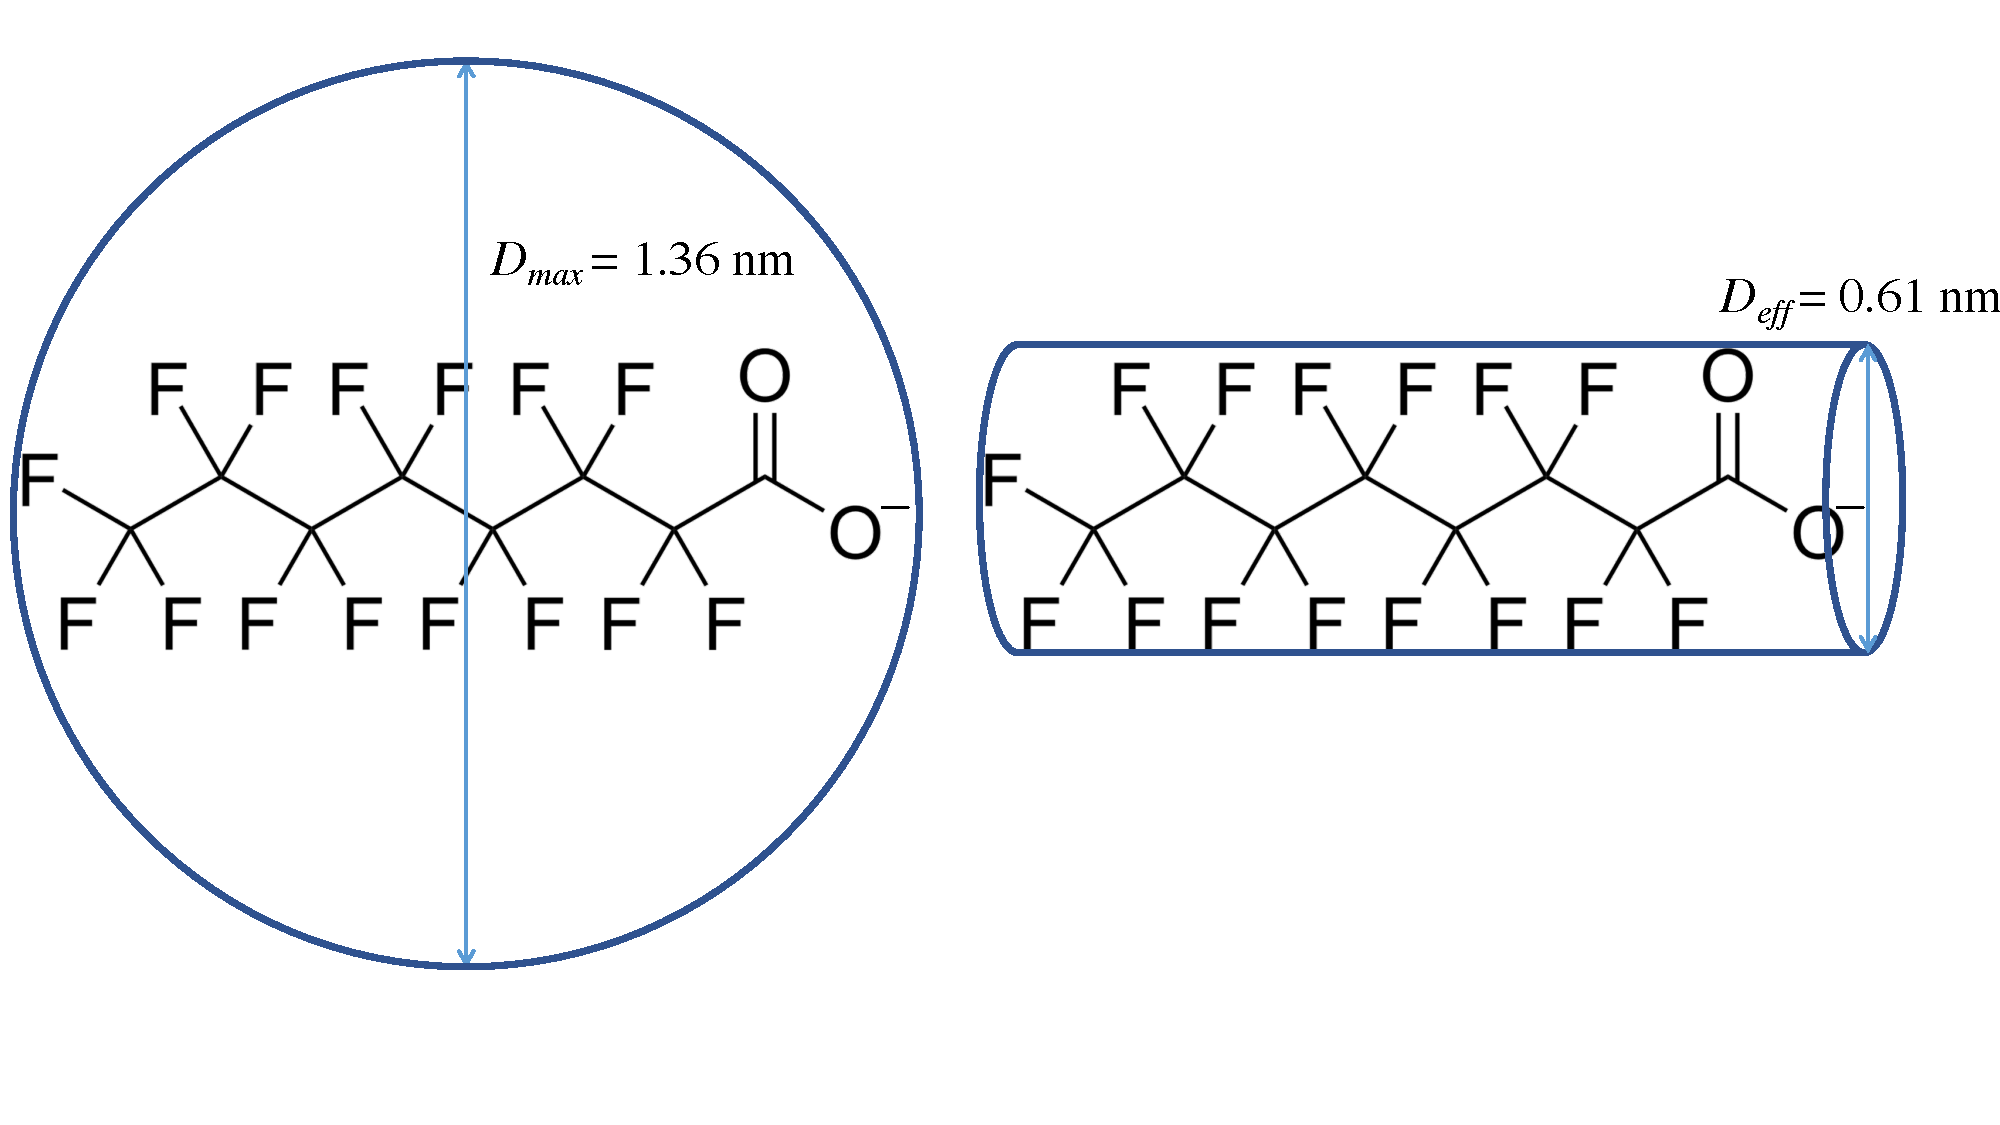
\includegraphics[width=0.8\textwidth, trim={0 2cm 0 0},clip]{Diagrams/Molecular_size.pdf}
    \caption{Definition of effective cross-sectional diameter ($D_{eff}$) and maximum diameter ($D_{max}$) shown for PFOA.}
    \label{fig:molecularSize}
\end{figure}

\subsubsection{Pore size distribution for pores $>$1.5 nm}
Similar to the trend for small pores, CWC also had the largest cumulative SA but the lowest PV for pores $>$1.5 nm (323 m\textsuperscript{2} g\textsuperscript{-1} versus 110 and 128 m\textsuperscript{2} g\textsuperscript{-1} for DSL and ULS, respectively). \cref{fig:PZD_large}a shows that the highest proportion of SA is allocated to pores between 1.5-3 nm for CWC and 1.5-5 nm for ULS and DSL. Cumulative PV is highest for ULS (0.126 cm\textsuperscript{3} g\textsuperscript{-1}), where PV for CWC was one order of magnitude lower (0.017 cm\textsuperscript{3} g\textsuperscript{-1}). Furthermore, the development of PV with pore diameter in \cref{fig:PZD_large}b shows a clear distinction between CWC and the two sewage sludge biochars. CWC has most of its PV in pores $<$3 nm, whereas PV for ULS and DSL steadily increase up to the maximum pore size of 35 nm. This difference becomes important for the SA/PV ratio seen in \cref{fig:PZD_large}c. Here, ULS and DSL have low and equivalent cumulative $\log~SA/PV$ ratios of 2.8 compared to the higher ratio of 3.2 for CWC (\cref{tab:SAPV}). Previous studies have consistently concluded that a large internal surface area and pore volume of adsorbents are the two most important parameters for achieving high sorption capacity of PFAS \citep{du2014adsorption,Sormo2021,Hale2016,ahmed2020per}. Similarly, the results of this study provide clear indications that a low SA/PV ratio can be considered a proxy for good PFAS sorption. The most plausible explanation for why CWC is the weakest sorbent among the three samples in this study is that CWC consists almost exclusively of micropores, whereas ULS and DSL also have pores in the mesopore range (2-50 nm). The shift observed by comparing SA and PV together demonstrates the importance of considering both pore size \textit{and} surface area when evaluating available sorption sites on biochar.

Since ULS and DSL had nearly equivalent SA/PV ratios, an additional parameter is needed to explain why ULS is a better sorbent than DSL (\cref{fig:PZD_large}c). Apart from SA and PV, carbon content has, in previous literature, been a good predictor of sorption affinity to PFAS \citep{Hale2016,Cornelissen2005}. ULS contains 29.6 \% carbon whereas DSL contains 13.5 \%.  

 This means that high porosity and sufficiently large pores are the two most important parameters that regulate high sorption capacity, and that the pore wall composition further contributes to enhanced sorption. 

\begin{figure}[htb]
    \centering
    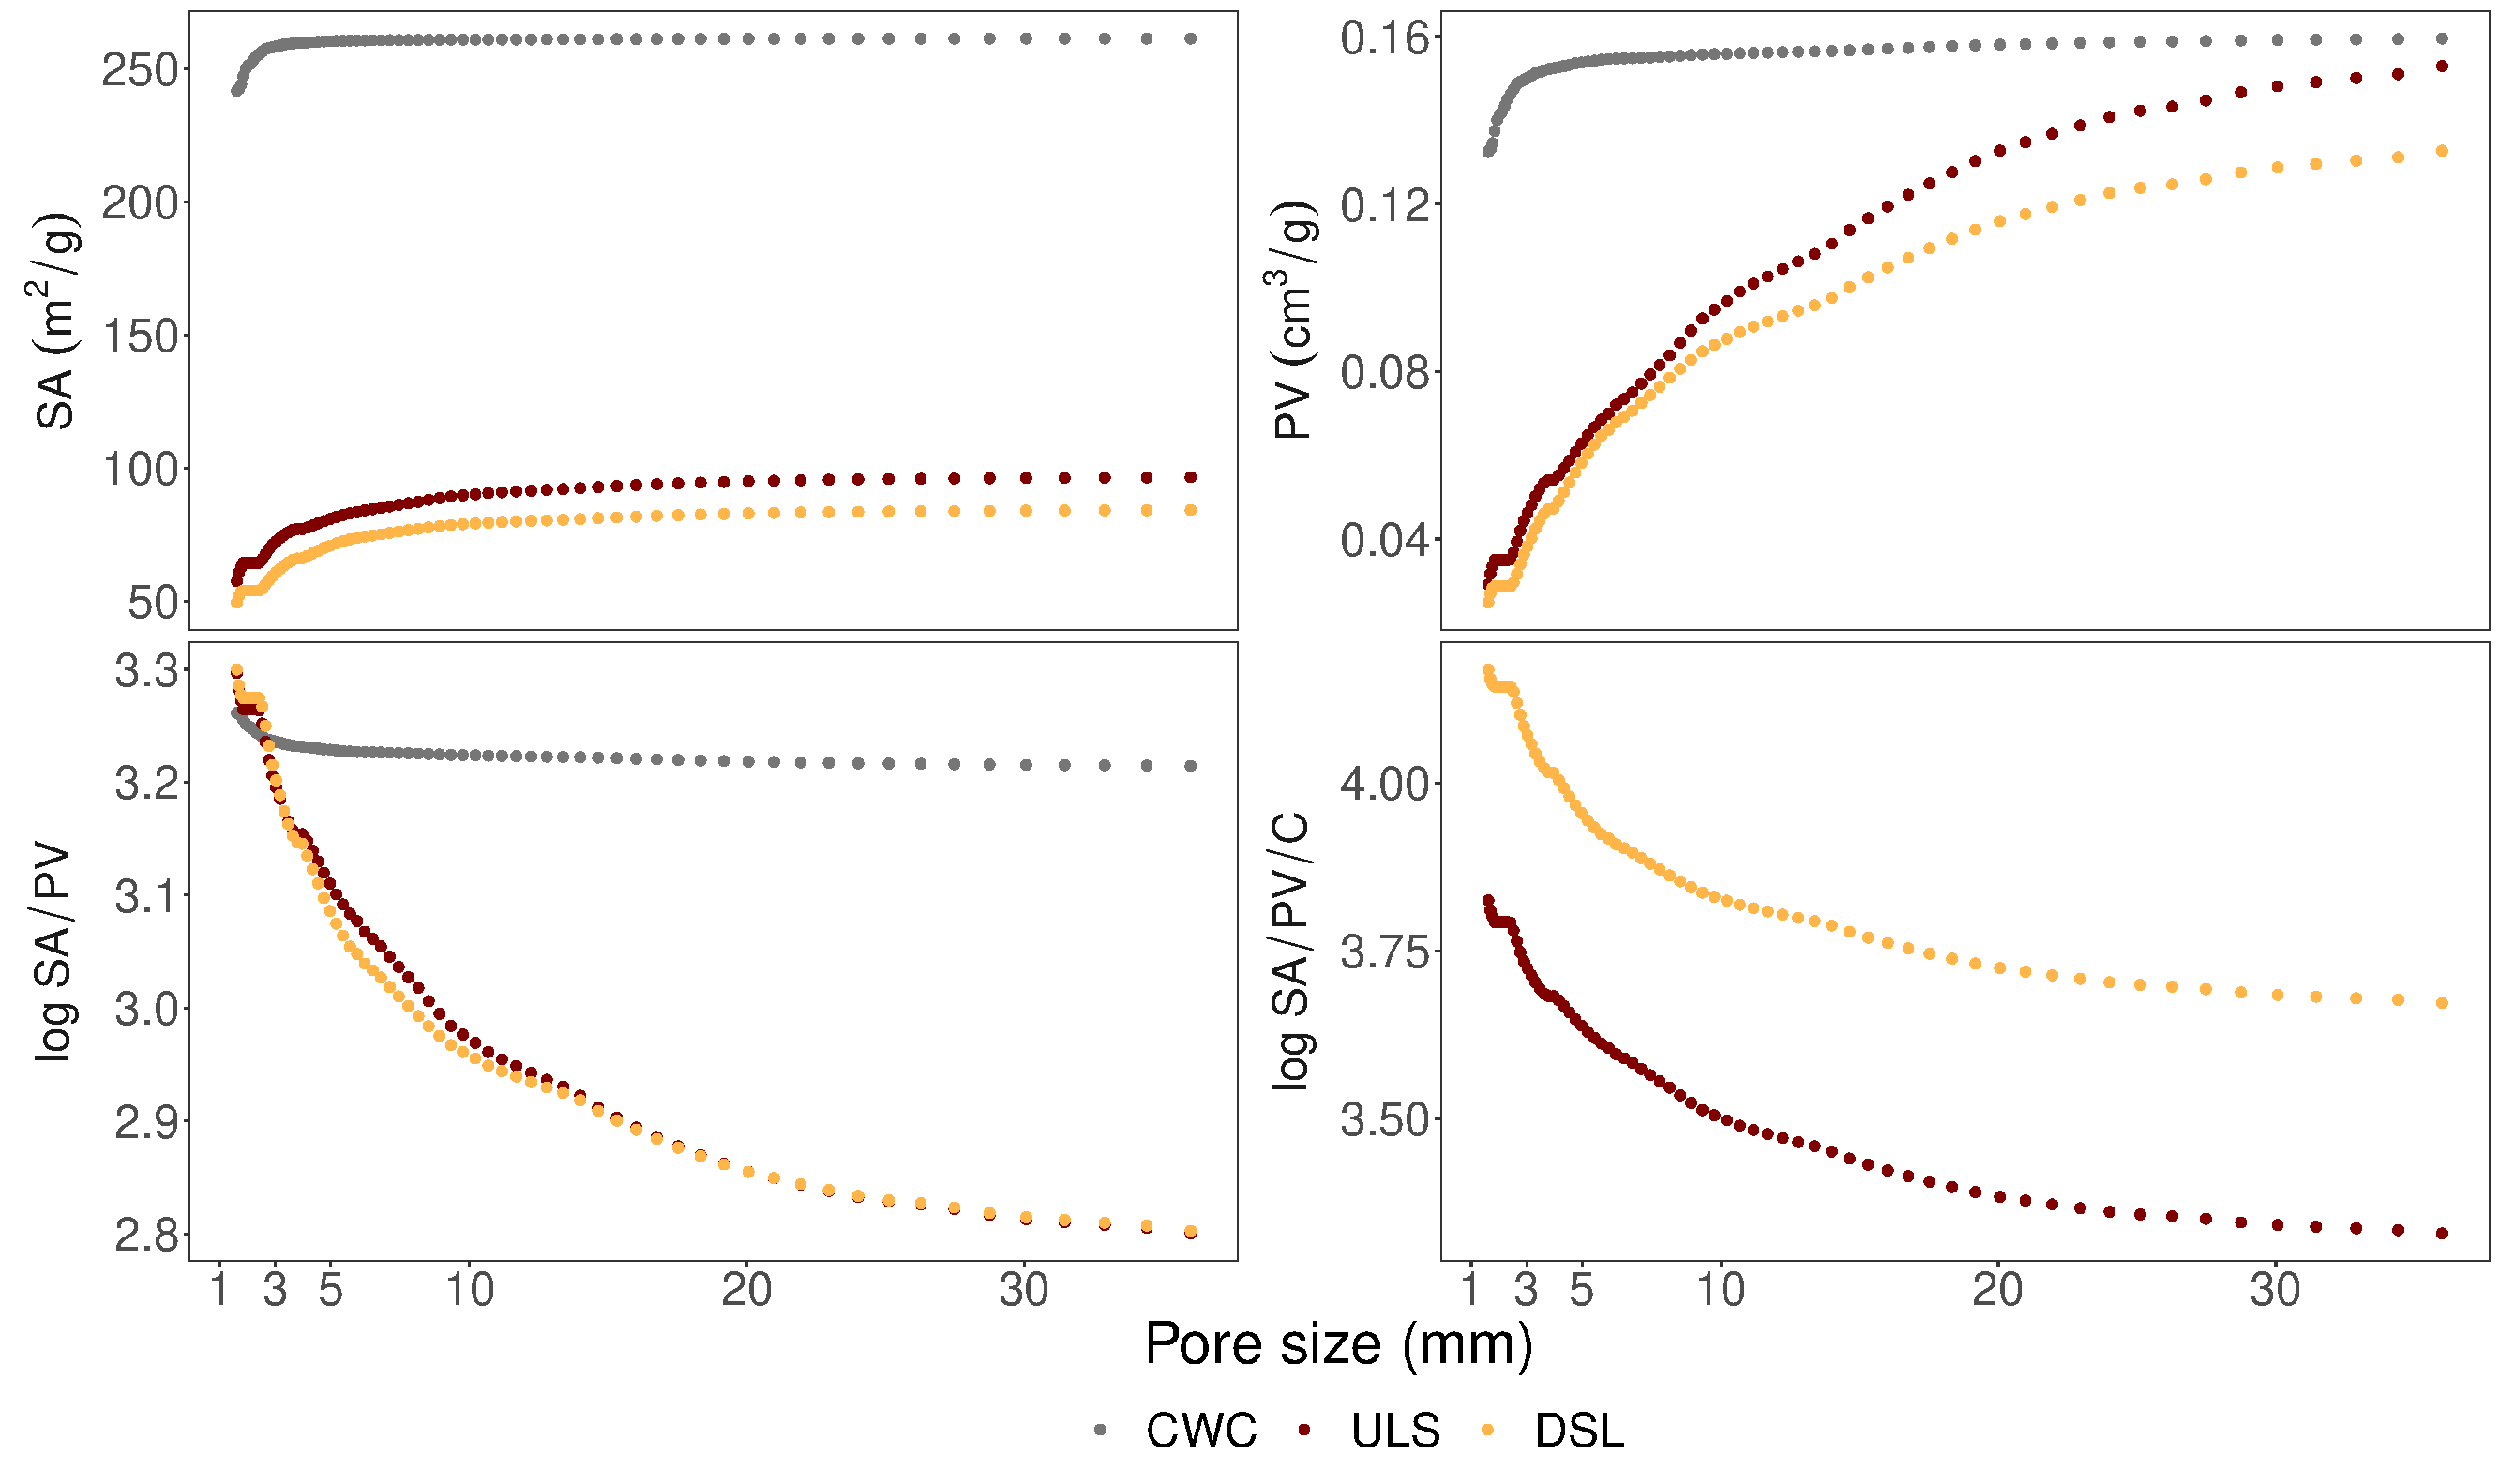
\includegraphics[width=\textwidth]{R/figs/PZD_SAPV_C_large.pdf}
    \caption{Cumulative pore size distribution for pores $>$ 1.5 nm using DFT theory. (a) Surface area, (b) pore volume, (c) SA/PV ratio for pores $>$1.5 nm normalized to carbon content (g C/g BC). (d) A lower SA/PV/C ratio indicates a higher degree of C in the pore wall matrix.}
    \label{fig:PZD_large}
\end{figure}

\subsection{Biochar surface chemistry}
A higher carbon fraction is commonly used as an indicator of biochar aromaticity and, thereby, higher possibility for hydrophobic interactions \citep{Cornelissen2005}. The higher sorption of PFCAs to the ULS and DSL biochars stand in contrast to findings in previous literature that consequently report that higher C-content is a good predictor for increased sorption \citep{fabregat2022examining}. However, previous PFAS sorption studies have been conducted on activated biochar and charcoal, more carbon-rich and porous feedstocks than biochar from sewage sludge \citep{Sormo2021, zhang2021sorption}. The effects of porosity will be discussed in \cref{sec:SAPV}. Despite lower carbon contents in the ULS and DSL biochars, this study supports previous literature that concluded that the importance of electrostatic interaction to sorption comes secondary to the hydrophobic effect. 

Surface hydrophobicity and degree of carbonization can be described by O/C, H/C, and N/C ratios \citep{chun2004compositions}. As reported previously, the O/C ratio of CWC (0.06) is within the same range as non-activated biochars pyrolyzed at 700\textdegree C \citep{LehmannAndJoseph2015, chun2004compositions,kupryianchyk2016biochar}. By contrast, the high oxygen content of DSL and ULS (61.4 and 57.1 \% respectively) results in increased O/C ratios of 4.6 and 1.9 respectively (\cref{tab:SAPV}). The difference between the O/C ratio \textless 1 for CWC compared to ratios \textgreater 1 for ULS and DSL indicate a significantly different degree of carbonization between the two feedstock types. At the same time, H/C ratios for all three biochar feedstocks are similar, and within the same range reported in previous literature \citep{chun2004compositions,kupryianchyk2016biochar}. 

A higher O/C and N/C ratio---indicative of more polar functional groups (hydroxyl, carbonyl, metal-containing groups, amines and amides)---has proven to be beneficial for PFAS sorption \citep{du2014adsorption,fabregat2022examining}. Researchers suggest several mechanisms related to surface polar groups that may contribute to enhanced sorption. First, basic functional groups such as amines have high $pK_a$s and are protonated at environmentally relevant pH providing anion exchange capacity and electrostatic attraction to the carboxylic acid heads \citep{deng2010removal}. Basic sites in \textpi-electron-rich, carbon-rich materials are important for PFAS sorption \citep{saeidi2020understanding}. N/C ratios for ULS and DSL are one order of magnitude higher than CWC. A high nitrogen/carbon (N/C) ratio can be indicative of more amine groups in the periphery of the condensed carbon structure. The positive charge on the nitrogen-containing functional groups can interact electrostatically with the PFCA carboxylate group. In addition, it is possible that they also engage in weak non-specific electrostatic interactions with the negative dipole of the CF-chain \citep{xiao2011effects}. The latter mechanism could explain the positive chain-length dependency on sorption seen for the sewage sludge biochars (\cref{fig:chainlength}) in addition to the low SA/PV/C ratio discussed in the previous section. Sewage sludge contains a homogeneous mixture of proteins and inorganic nutrients that will denaturate in some form during thermal treatment. To the author's knowledge, no data exists on how speciation of nitrogen changes during pyrolysis. Even though a higher N/C ratio is only an indication for nitrogen functional groups, the presence of amines is likely.

\begin{table}
\centering
\caption{Mean pH ($\pm$ standard error) measurements for the different batch test slurries (n=3) where S is soil and BC/S/L is the biochar:soil:liquid ratio.}
\label{tab:pHcond}
\begin{tabular}{lcc}
\toprule
Biochar & \multicolumn{1}{c}{pH} & BC/S/L\\ \midrule
ULS   & 7.10 ± 0.03 & 1/0/500\\
DSL   & 7.31 ± 0.01 & 1/0/500\\
CWC   & 7.36 ± 0.04 & 1/0/500\\
ULS+S & 7.18 ± 0.01 & 1/50/500\\
DSL+S & 7.14 ± 0.00 & 1/50/500\\
CWC+S & 7.09 ± 0.03 & 1/50/500\\
S     & 7.08 ± 0.03 & 0/1/10\\
\bottomrule
\end{tabular}
\end{table}


\subsubsection{Electrostatic interactions---effect of solution and biochar surface chemistry \label{sec:inorganic}} 
Solution chemistry, pH, and composition of elements other than C, O, H and N may provide further insight into how the pore walls of CWC, ULS and DSL differ from one another, and how these elements can influence sorption. pH varied little across sample types with an average pH of 7.18 $\pm$ 0.02 (\cref{tab:pHcond}). Therefore, pH of the biochar-water batch tests slurries have only been used to discuss expected surface charges. In the environment, the carboxylic functional group of PFCAs is negatively charged due to the strong electron withdrawing fluorine atoms \citep{goss2008pKa}. Surface charges for biochar is pH-dependent and is usually negatively charged at neutral pH \citep{zhang2013sorption}, which was the case for the batch tests in the present study. However, point of zero charge measurements for the biochars did not become available in time for incorporation in this discussion. Therefore, a net negative biochar surface is assumed but not confirmed.

In this study, highest sorption was seen for the biochars that had the highest composition of elements other than C, O, H, and N. CWC biochar contained only 1.4\% other elements whereas the sludge biochars, ULS and DSL, contained substantially more (10.9\% and 23.2\% respectively). A table with the total biochar elemental composition is given in \cref{appSec:elements}. Some of these elements are commonly found as freely dissolved ions. Since dissolved ions were not analyzed, we can only assume that, at large, the alkalis (K and Na) and earth alkalis (Mg and Ca) are present as dissolved cations originating from the biochar ashes, whereas it is likely that Fe is predominantly incorporated in the biochar matrix. Iron speciation will be further discussed in \cref{sec:Fe}. The higher content of other elements than C, H, O, and N in ULS and DSL suggests that sorption of PFCAs onto the sludge chars were likely influenced by the presence of charged species, both in solution and on the biochar surface. Coexisting inorganic ions complicate the sorption behavior of PFCAs because sorption can both be suppressed and enhanced by different electrostatic mechanisms \citep{du2014adsorption} which will be discussed below. 

Sorption can be suppressed by electrostatic repulsion of the carboxylate group on PFCA by the negatively charged biochar surface, or by competitive sorption of anions to positive BC sites \citep{sigmund2022sorption}. Electrostatic repulsion can explain why $K_F$-values were lowest for the shorter-chain PFCAs (\cref{tab:summary_stats_single}). The repulsion effect becomes weaker for the longer-chain PFCAs where the hydrophobic effect gets more dominant. Electrostatic repulsion is reduced at lower pH because more negative BC sites are protonated, called surface-charge neutralization \citep{zhang2013sorption}. This allows for PFCA anion- \textpi-bond interaction with biochar \citep{sigmund2022sorption}. Sorption can be enhanced through electrostatic attraction to positively charged BC functional groups and divalent cation bridging \citep{du2014adsorption}. Cation bridging is the electrostatic linking of negatively charged PFCAs to negatively charged biochar surfaces by a divalent ion that "bridges" them together \citep{sigmund2022sorption}. Common divalent ions present in biochar ash that contribute to bridging are Ca\textsuperscript{2+} and Mg\textsuperscript{2+}. Composition of Ca\textsuperscript{2+} and Mg\textsuperscript{2+} was three to six times higher in the sludge biochars compared to CWC biochar (\cref{tab:BC_mainElements}. Bridging has been shown to be an important sorption mechanism in, for example, sediments, mineral materials, and black carbon \citep{higgins2006sorption}. Apart from bridging between the BC surface and PFAS functional groups, divalent ions can chain individual PFAS molecules together \citep{wang2011}. This creates an even more hydrophobic complex that can sorb more strongly to biochar. More frequent formation of divalent cation bridges for the ULS and DSL biochars is therefore expected. Although sorption \textit{capacity} has not been measured directly, the above-mentioned mechanisms for PFAS interaction with charged and polar functional groups may be contributors to the higher sorption found for the more heterogeneous, mineral-rich matrices of the sewage sludge biochars.

The positive correlation between $\log~K_F$ and chain length for all three biochars in this study (\cref{fig:chainlength}) indicates that electrostatic interactions play a minor role for sorption to these biochars. If electrostatic interactions played an equally important role as hydrophobic interactions, sorption across PFCA chain lengths would be more similar because electrostatic attraction would become increasingly energetically favorable with shorter chain length. 

\begin{table}
\centering
\caption{Composition of a selection of elements in the biochar samples in g/kg.}
\label{tab:BC_mainElements}
\begin{tabular}{lrrrrrrrr} \toprule
 & Ca & Fe & K & Mg & Na & P & S & Si \\ \midrule
CWC & 8 & 0.1 & 4.0 & 0.9 & 0.05 & 0.4 & 0.09 & 0.2 \\
DSL & 26 & 180 & 3.7 & 4.7 & 1.8 & 8.0 & 7.2 & 0.6 \\
ULS & 21 & 23 & 6.8 & 5.3 & 2.4 & 45 & 2.9 & 1.7 \\ \bottomrule
\end{tabular}
\end{table}

\subsubsection{Iron speciation\label{sec:Fe}}
Due to the lack of corresponding reference compounds for some of the EXAFS signals, no satisfying fit was obtained for the iron species present in the sewage sludge biochar samples. This information indicates that iron is not only present as iron oxides. The Fe K-edge XANES spectra (\cref{appFig:valence}) and EXAFS spectra (\cref{appFig:Fe_species}) show that DSL and ULS are similar in valence and speciation. They mainly consist of reduced forms of Fe (Fe(II)), and DLS is slightly more reduced than ULS. Total Fe concentration is especially high for DSL (180 mg/kg, \cref{tab:BC_mainElements}), making up as much as 18\% of its matrix (3.3\% and 0.01\% for ULS and CWC respectively). The Fe concentration will therefore significantly affect surface morphology of DSL. PFAS has been shown to form inner-sphere complexes via covalent metal-ligand bonds (Fe-carboxylate) by means of the following reaction \citep{du2014adsorption}:

\begin{equation}
    \mathrm{\equiv Fe-OH_2^+ ~ + ~ CF_3(CF_2)_nCOO^- \rightarrow ~ \equiv Fe-OOC(CF_2)_nCF_3 ~+~ H_2O}
\end{equation}

where the triple bond represents chelation of Fe to the biochar matrix. Point of zero charge (pzc) for Fe(oxyhydr)oxides, such as ferrihydrite and goethite, are around 7, similar to the solution pH measured for the water-biochar systems (see \cref{sec:inorganic}). The iron species are expected to be neutral for the systems analyzed and will likely not be one of the dominating sorption mechanisms for PFCA. 

%%%%%%%%%%%%%%%%%%%%%%%%%%%%%%%%%%%%%%%%%%%%%%%%%%%%%%%%%%%%%%%%%%%%%%%%%%%%%%%%%%%%%%%%%%%%%%%%%%%%%%%%%%%%%%%%%%%%%
%%%%%%%%%%%%%%%%%%%%%%%%%%%%%%%%%%%%%%%%%%%%%%%%%%%%%%%%%%%%%%%%%%%%%%%%%%%%%%%%%%%%%%%%%%%%%%%%%%%%%%%%%%%%%%%%%%%%%
%%%%%%%%%%%%%%%%%%%%%%%%%%%%%%%%%%%%%%%%%%%%%%%%%%%%%%%%%%%%%%%%%%%%%%%%%%%%%%%%%%%%%%%%%%%%%%%%%%%%%%%%%%%%%%%%%%%%%

\section{Sorption attenuation by soil and PFCA cocktail}
This section discusses sorption attenuation for the different batch test categories that were prepared (\cref{fig:batchtests_flowchart}). The categories were: 

\begin{itemize}
    \item \textbf{BC single}: biochar-water spiked with single PFCAs
    \item \textbf{BC mixed}: biochar-water spiked with a PFCA cocktail
    \item \textbf{BC soil single}: soil-biochar-water spiked with single PFCAs
    \item \textbf{BC soil mixed}: soil-biochar-water spiked with a PFCA cocktail
    \item \textbf{Soil single}: soil-water spiked with single PFCAs
    \item \textbf{Soil mixed}: soil-water spiked with a PFCA cocktail
\end{itemize}

\cref{subfig:C10} shows the $K_d$-values for the different batch test categories spiked with the same concentration of each compound at the highest spike point, SC10 (\cref{tab:spikeConcentrations}). This way of comparing partitioning of the same compound across biochar samples was decided to be the simplest because the overall mass PFCA added to the system was the same for all samples. $K_d$ for the biochar-soil batch tests has not been corrected for the amount sorbed by soil itself due to inconsistent results for the $K_d$ in soil (\cref{tab:attenuation}). Therefore, $K_d$ for BC soil single, BC soil mixed and BC mixed represent the collective partitioning coefficients for biochar and soil. However, the sandy soil used has low sorption strength, with a mean $\log~K_d$ value of 2.47, over 1000 times lower than for, e.g., singly-spiked PFDA to ULS-water (6.06). thus, the effect of this was relatively limited. The cocktail consisted of 2.5\% PFPeA, 7.7\% PFHxA, 1.4\% PFHpA, 18.2\% PFOA, 21.3\% PFNA, and 48.8\% PFDA. Since the cocktail consisted of different concentrations of each compound, a trend for attenuation with chain length cannot be derived. However, the relative $K_d$-values of each batch test category, as well as comparisons between biochar samples, yield interesting results. 

In \cref{subfig:C10}, the difference in $\log~K_d$ between BC single and the other sample types equates to how much sorption is attenuated in the presence of soil and/or other PFCAs. Fouling, together with attenuation, are terms used to discuss the weakening of sorbent sorption by natural organic matter or competing contaminants \citep{Werner2006}. For all compounds, the presence of other PFCAs was responsible for the highest drop in $\log~K_d$, consistent with the findings of \cite{Cornelissen2006}. Overall, $\log~K_d$ decreased in the following order: BC single $>$ BC soil single $>$ BC mixed $>$ BC soil mixed $>$ soil single and mixed. Attenuation appears to be similar for all biochars as the points for each batch type align parallel for PFOA, PFNA, and PFDA. This trend shows that the mixed systems have greatest attenuation, where sorption is up to two orders of magnitude weaker than BC single, the reference of calculating the AFs. This means that sorption is non-linear at high concentrations, something which will be discussed further in \cref{sec:non-linearity}. These results are in line with previous literature \citep{deng2010removal, zhou2010sorption}.

\subsection{Attenuation factors}
\cref{subfig:AF} shows the attenuation factors (\acrshort{AF}) for each batch test category, defined as:

\begin{equation} \label{eq:AF}
    AF = \frac{K_{d,BC single}}{K_{d,x}}
\end{equation}

where $K_{d,BC~single}$ is the mixed, soil mixed, or soil single batch test sample partition coefficient. AFs for PFPeA, PFHxA and PFHpA are not presented due to lack of consistent results. Lowest AFs were measured for BC-soil-PFOA, where AFs were 3, 4, and 10 for CWC, DSL, and ULS respectively. All calculated AFs are in \cref{tab:attenuation}. 

\begin{table}
\centering
\caption{Attenuation factors (AF) calculated as $K_{d,BC~single}/K_{d,x}$}
\label{tab:attenuation}
\begin{tabular}{llrrrrrr} \toprule
 &  & \multicolumn{2}{c}{CWC} & \multicolumn{2}{c}{DSL} & \multicolumn{2}{c}{ULS} \\ \cmidrule(l){3-4} \cmidrule(l){5-6} \cmidrule(l){7-8}
Compound & type & $\log~K_d$ & AF & $\log~K_d$ & AF & $\log~K_d$ & AF \\ \midrule
PFOA & BC mix & 2.84 & 6 & 3.17 & 23 & 4.13 & 29 \\
PFNA & BC mix & 2.33 & 109 & 3.03 & 140 & 4.40 & 29 \\
PFDA & BC mix & 2.95 & 9 & 3.60 & 32 & 5.09 & 9 \\ \addlinespace \hline \addlinespace
PFOA & BC S mix & 2.73 & 8 & 3.24 & 19 & 3.47 & 134 \\
PFNA & BC S mix & 2.68 & 48 & 3.33 & 71 & 3.73 & 138 \\
PFDA & BC S mix & 2.91 & 10 & 3.67 & 27 & 4.16 & 78 \\ \addlinespace \hline \addlinespace
PFOA & BC S single & 3.19 & 3 & 3.98 & 4 & 4.61 & 10 \\ \bottomrule
\end{tabular}
\end{table}

Highest attenuation were measured for the cocktail samples, with minor variance between the BC soil mixed and BC mixed samples. Attenuation factors are in the range 6-140 which means that sorption has been reduced by 84-99\%. This suggests that the total concentration of the cocktail is responsible for saturating sorption sites almost completely, and that the presence of soil in this case does not contribute to additional fouling. These factors are very high due to five other compounds added at similar concentrations. Overall, \cref{fig:C10_AF} shows that attenuation by the cocktail is more significant than attenuation by soil. This can mean two things: 1) The soil does not block biochar sorption sites, or 2) The soil, which has a $\log~K_d$ of 2.6 $\pm$ 2.0, sorbs some of the PFCAs that have been blocked from sorption onto the biochar. It was difficult to evaluate any trends in AFs between biochar samples or PFCA chain lengths. Further investigations by conducting attenuation experiments with a larger biochar sample size are needed to determine a relationship between biochar properties and fouling. 

Colored filtrate and humus aggregation seen during analysis of the soil batch tests indicate that sorption of organic matter (OM) to biochar is likely (see \cref{sec:S-BC}. The soil used was a sandy soil with 1.3 \% TOC (details on soil properties is in \cref{sec:Soil}). By the co-existence of OM and dissolved organic carbon (DOC), sorption attenuation occurs by a combination of competitive and weaker sorption of PFAS to OM and DOC, and the competitive sorption of OM to biochar. Large humic acids (300-600 nm) clog the pores, preventing diffusion of PFAS \citep{Cornelissen2006,kluvcakova2018size}. Furthermore, the size of the organic molecules is a critical factor as humic molecules whose size is similar to that of PFAS are responsible for the highest competition \citep{du2014adsorption}. Given that size fractionation was not investigated in this study, the effect of differences of size for humic acids can only be discussed in theory.

\begin{figure}
    \centering
        \begin{subfigure}[]{\linewidth}
            \centering
            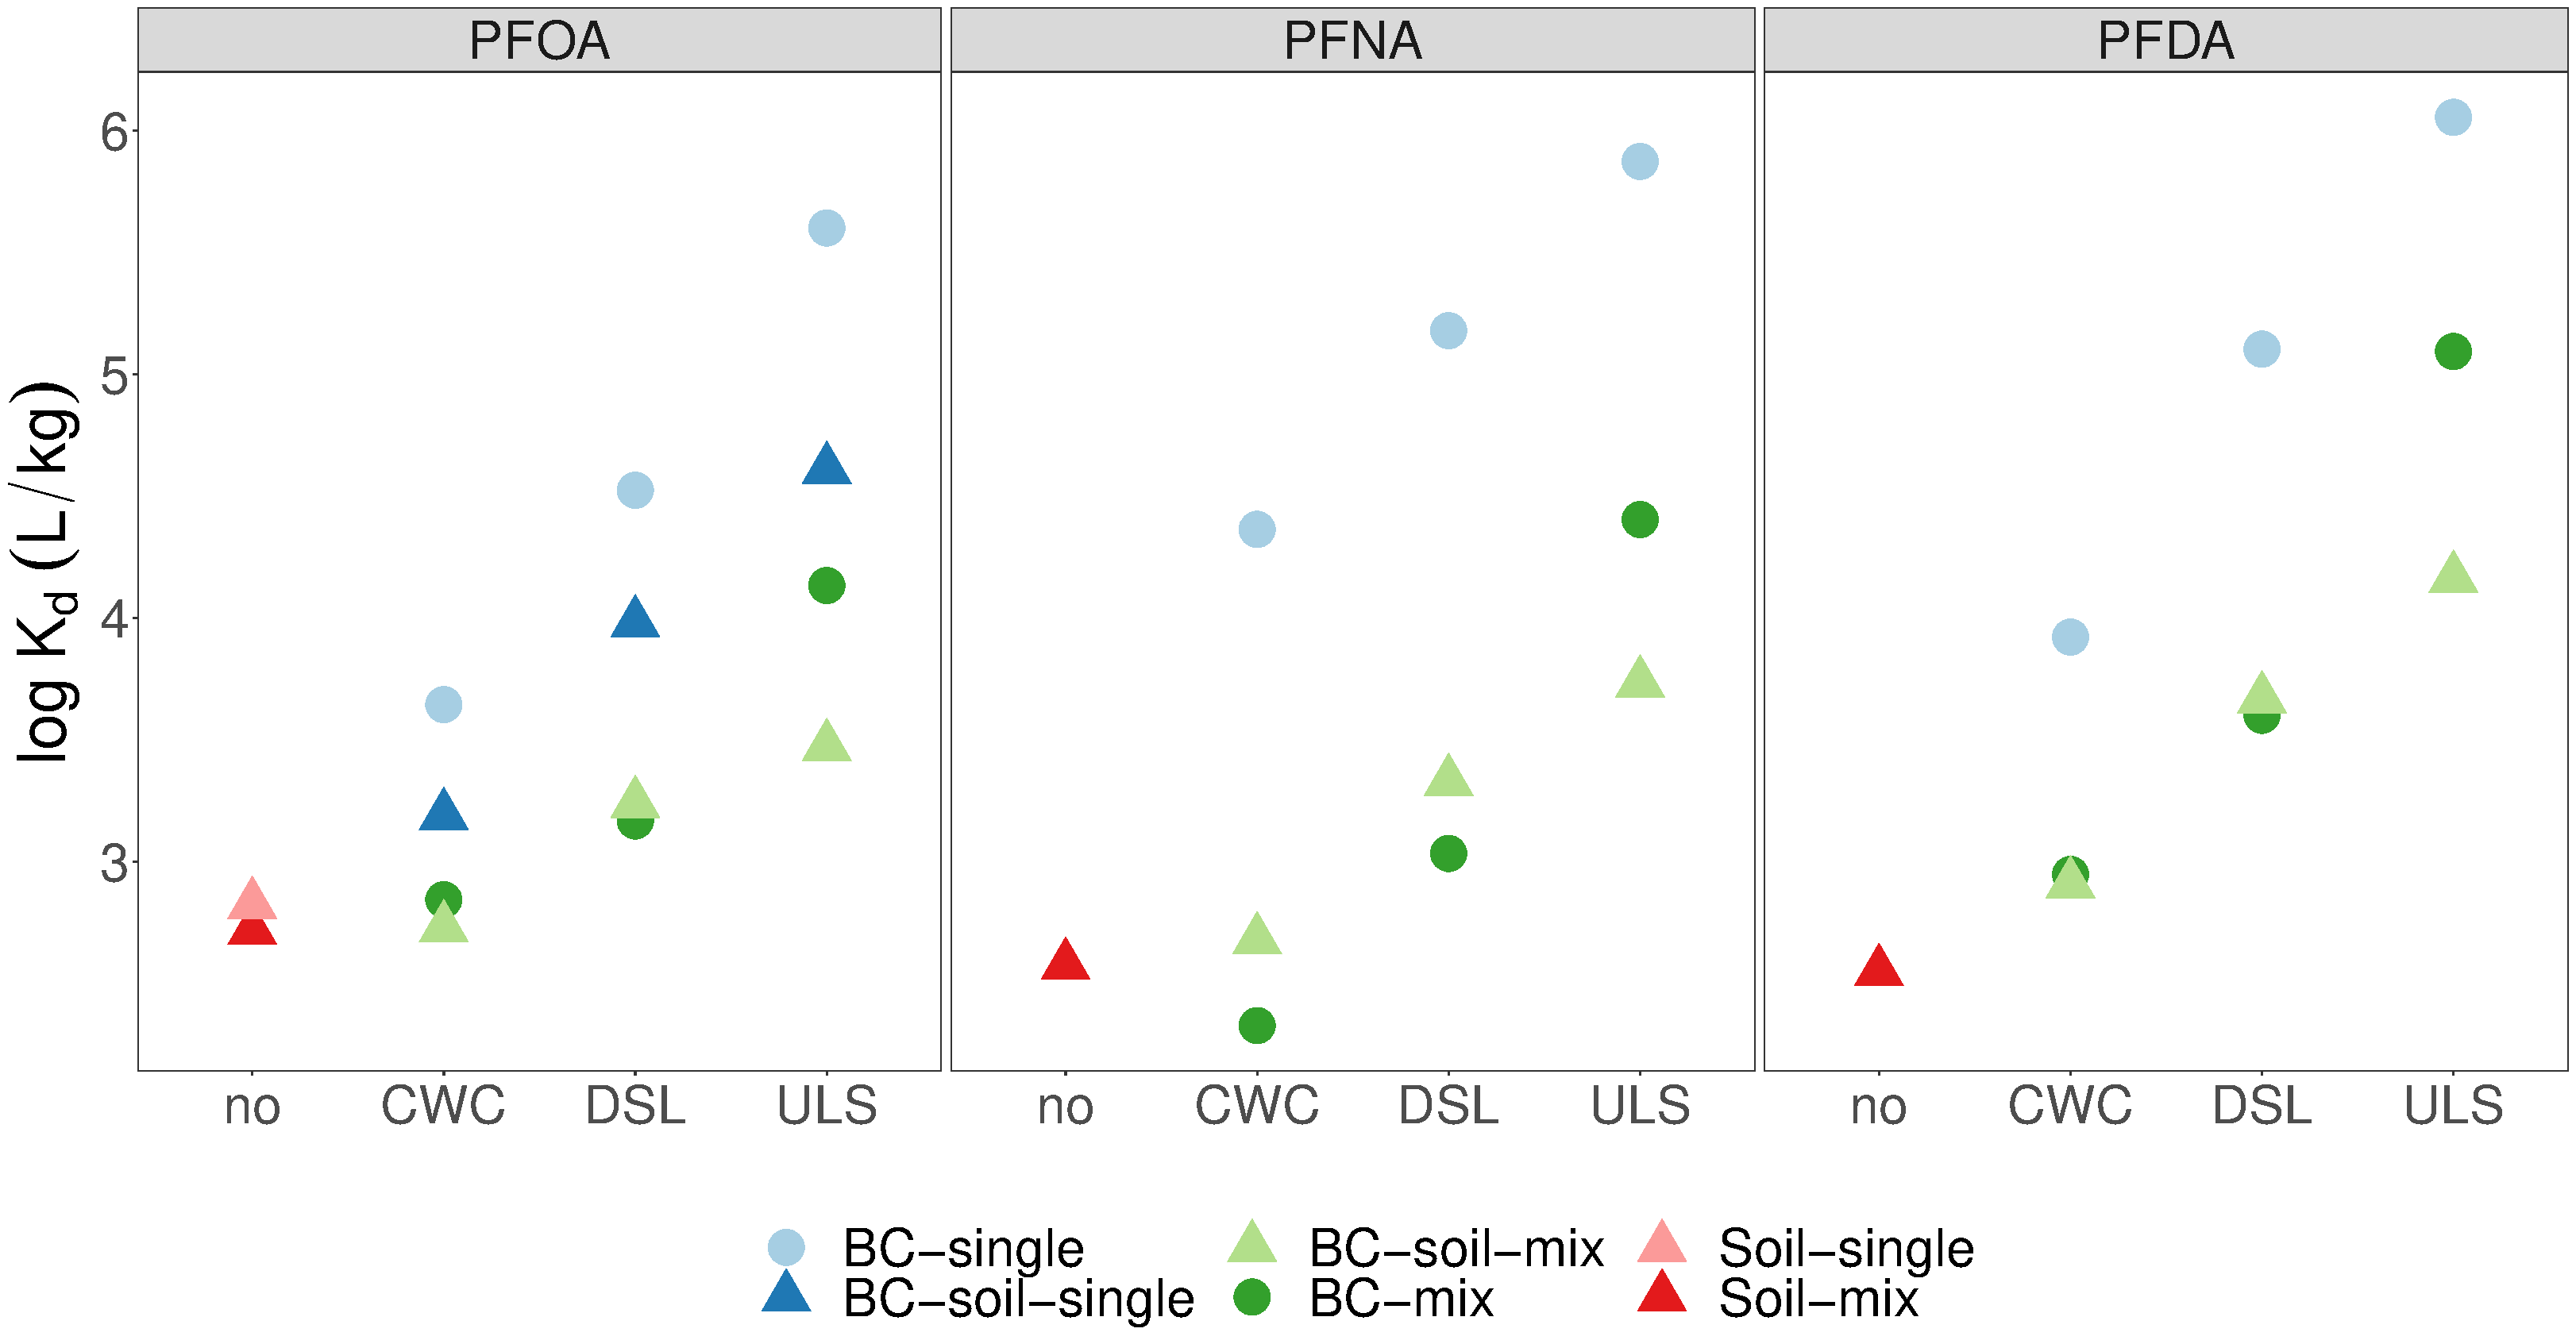
\includegraphics[width=0.75\textwidth]{R/figs/C10.pdf}
            \subcaption{$\log~K_d$ for PFOA, PFNA, and PFDA spiked at SC10 (1 953, 1 409, and 3 830 \textmu g L\textsuperscript{-1} respectively) for the different biochar feedstocks (CWC, DSL, ULS) and soil only (no biochar).}
            \label{subfig:C10}
        \end{subfigure}
        \begin{subfigure}[]{\linewidth}
            \centering
            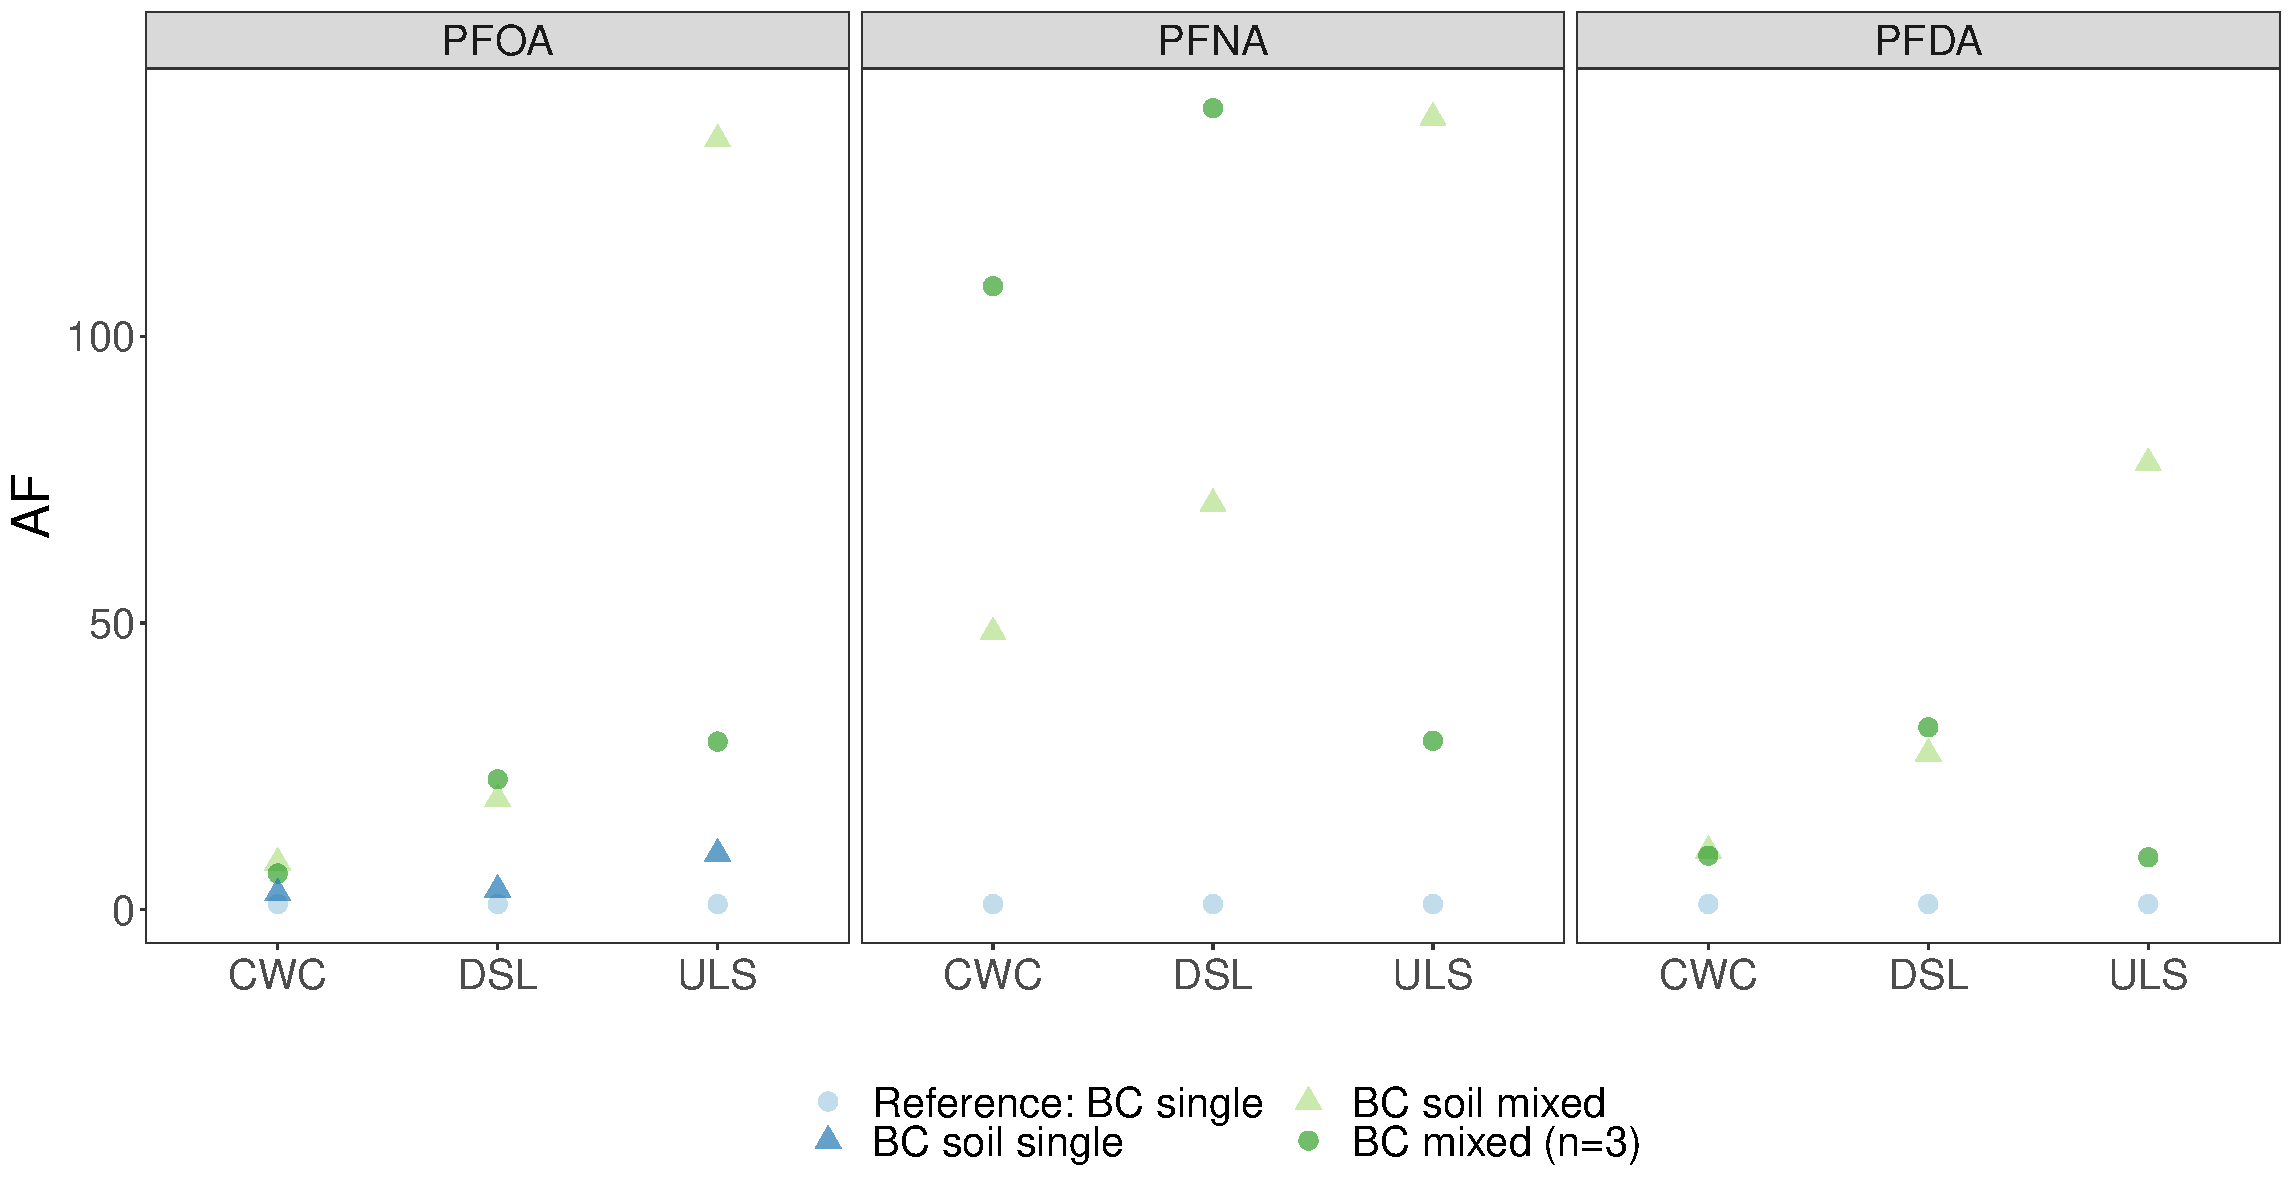
\includegraphics[width=0.75\textwidth]{R/figs/Attenuation_factors_C10_OND.pdf}
            \subcaption{Attenuation factors (AF) at SC10 for PFOA, PFNA, and PFDA calculated as $K_{d,BC single}/K_{d,x}$ where $K_{d,x}$ are the batch test categories. BC cocktails are spiked with 7.8 mg/L total PFCA and BC soil cocktails with 10.8 mg/L (the difference is explained in the corresponding section). See \cref{tab:spikeConcentrations} for spike concentrations used for each PFCA in the single-spike and cocktail-spike batch tests.}
            \label{subfig:AF}
        \end{subfigure}  
    \caption{Reduction in \textbf{(a)} $\log~K_d$ at SC10 and \textbf{(b)} attenuation factors at SC10.}
    \label{fig:C10_AF}
\end{figure}

\subsection{Sorption attenuation of PFOA isotherms}
\cref{fig:PFOA_attenuation} shows the effect of attenuation on the PFOA isotherms for BC soil single and BC soil mixed. The isotherms were spiked with the same $C_i$ as BC single, but only six of the ten points were selected for the attenuation isotherms (\cref{sec:S-BC}. For all biochars, BC single has the highest sorption, followed by BC soil single, and BC soil mixed. This trend gives a good indication of the order of factors that influence attenuation, and is consistent with the results discussed earlier in this section. The isotherms have similar $C_s$ concentrations, but varying $C_w$, depending on sample type. Due to pore blocking and competitive sorption by natural organic matter and xxxx, more sorbate in solution is needed to push the same amount of molecules onto the solid phase in the presence of soil. This effect can be further enhanced by the presence of both soil and a cocktail since this isotherm has the highest $C_w$ and lowest $C_s$. This is due to the fact that PFCAs with longer chain lengths (PFNA and PFDA) have an advantage over PFOA when competing for sorption sites \citep{Sormo2021}. Consistent with \cref{fig:C10_AF}, the cocktail attenuation effect is more significant than attenuation by soil. Parallel isotherms mean that attenuation is the same across the whole concentration range, as, for instance, between BC single and BC soil single for ULS. For some isotherms, attenuation is minimal at low concentrations and increases with increasing spike concentration. This is the case for the DSL isotherms, something that can be explained by the non-linear sorption at higher concentrations. So, when spike concentration increases, sorption attenuation also increases. 

\begin{figure}[htb]
    \centering
    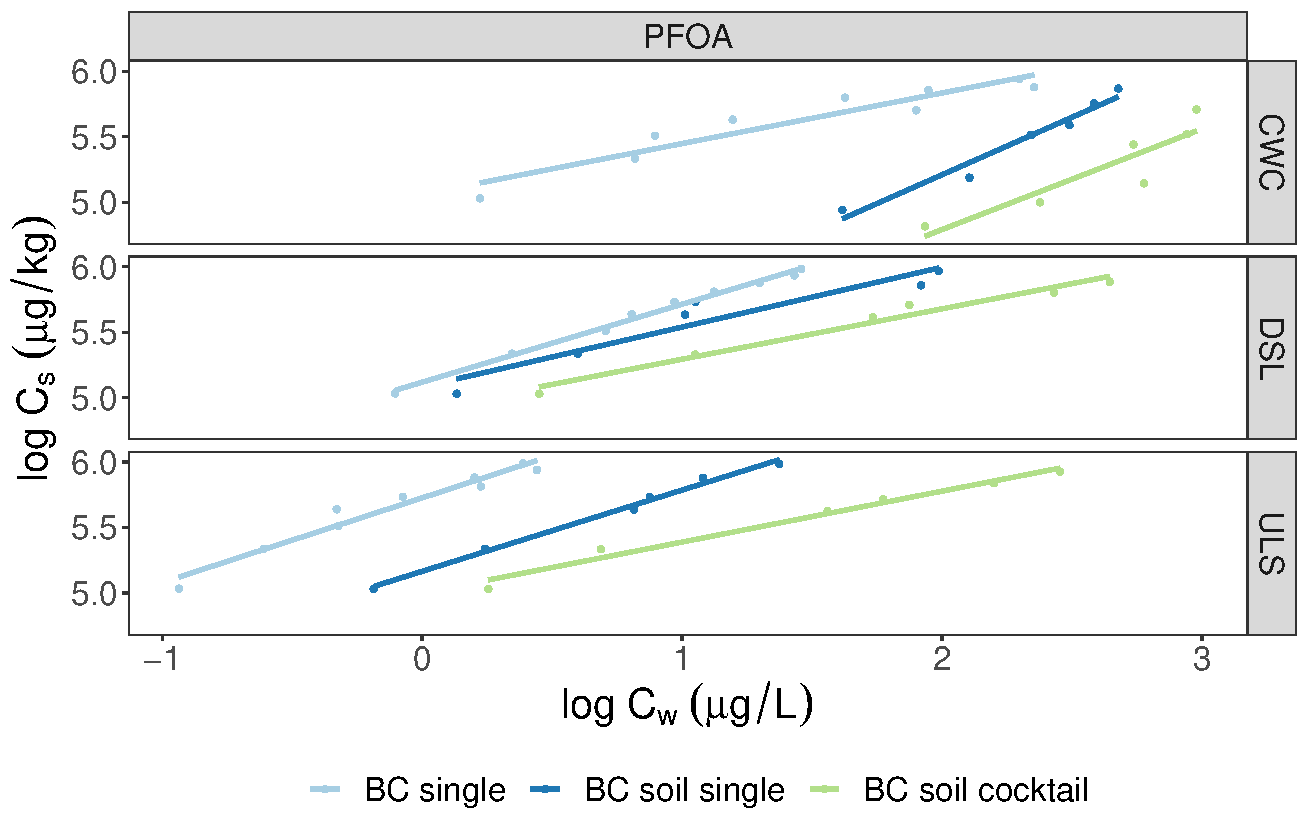
\includegraphics[width=0.8\textwidth]{R/figs/Attenuation_isotherms_PFOA.pdf}
    \caption{Sorption isotherm comparison for PFOA single-compound spike in biochar (BC single), single-compound spike in soil-biochar (BC soil single), and PFOA spiked in a cocktail in soil-biochar showing attenuation by soil and competing congeners.}
    \label{fig:PFOA_attenuation}
\end{figure}

\subsection{Freundlich sorption non-linearity}\label{sec:non-linearity}
The non-linear sorption isotherms for PFOA in \cref{fig:PFOA_nonlinear} shows how sorption is attenuated at higher concentrations, and how attenuation changes in the presence of soil and soil with other PFCAs. When a linear model is derived from applying the $\log$ of each axis, the slope ($n_F$) represents how linear the isotherm is within the concentration interval achieved (\cref{sec:models}). The resulting Freundlich coefficients ($\log~K_F$ and $n_F$) for PFOA are given in \cref{tab:PFOA_Freundlich}, and the remaining compounds are in \cref{appSec:Sorption}\cref{apptab:summary_stats_all}. Two general conclusions can be drawn from these figures: 1) Attenuation is higher in the presence of soil, and even higher when soil and cocktail are added together. And 2) The concentration ranges for some of the isotherms are too narrow to properly determine representative Freundlich coefficients for a wider concentration range. Therefore, conversion of $\log~K_F$ to either higher or lower units will be associated with greater uncertainty. 

All BC single isotherms have $n_F<1$. This indicates that the concentration interval achieved shows some degree of attenuation (\cref{tab:summary_stats_single}. This is consistent with other studies where sorption to biochar have $n_F$-values, typically, around 0.3-0.7 \citep{Cornelissen2005}. Both concentration interval and $n_F$ should be considered together in order to make suggestions about the sorption capacity of biochars. \cref{fig:nonlinear_OND} shows the non-linear BC-single isotherms for PFOA, PFNA and PFDA, where the degree of non-linearity is more easily visualized than the $n_F$-values alone. For example, \cref{fig:nonlinear_OND} shows that the CWC isotherms have more attenuation than DSL and ULS, and that $C_w$s have measurements across a wider concentration range. This is consistent with the lower $\log~K_F$s found for CWC. \cref{fig:nonlinear_OND} also shows that the isotherms for PFNA-DSL and PFNA-ULS are nearly linear, and span aqueous concentrations only within the same order of magnitude. Higher spike concentrations, or lower BC dosages, should have been used in order to get isotherms that cover the regions of attenuated sorption for these biochars and compounds. However, this information itself indicates that sludge biochars have higher sorption capacities than CWC.  

The concentration range achieved for $C_w$ for the sorption isotherms was an average of 1.3 $\log$ units, in contrast to the desired concentration range over 4 $\log$ units. Poor signals were achieved for the SC1 points and were removed from the data analysis. This resulted in the spike concentration interval being reduced to two orders of magnitude (\cref{tab:spikeConcentrations}). In retrospect, spike concentrations at each $\log$ unit should have been selected instead of spreading the ten concentrations evenly across the concentration range. For the short-chain compounds (PFPeA and PFHxA), correlations were poor. This resulted in higher standard errors, and some slopes that have $n_F>1$, which is unrealistic (PFHxA-DSL: n=1.11 and PFHpA-ULS: 1.08). However, the standard error is also high ($\pm$ 0.11 for both) and can account for this abnormality. Poor sorption strength of PFPeA and PFHxA to biochar may explain the poor correlations. The CWC isotherms had the widest concentration intervals for $C_w$. This can be understood by the fact that CWC is the weakest sorbent of the three biochars studied.  

Electrostatic interactions between PFCAs and sediment can contribute to enhancing saturation of the adsorption sites as well as intermolecular electrostatic repulsion between individual molecules \citep{higgins2006sorption,yin2022insights}. \cite{yin2022insights} presents two main explanations for why sorption of PFCAs to biochar is non-linear: 1) successive saturation of adsorption sites, and 2) the complex composition of biochar with negative, positive and neutral charges within same matrix. 

\begin{table}
\caption{Freundlich sorption parameters and standard errors for the PFOA isotherms. Freundlich coefficients for the soil samples are the collective partition coefficients for soil and biochar because $K_d$ for soil alone was not accurate enough. All $K_F$ data are in units of $\mathrm{(\mu g/kg)/(\mu g/L)^{n_F}}$.}
\centering
\adjustbox{max width=\textwidth}{%
\begin{threeparttable}
\label{tab:PFOA_Freundlich}
\begin{tabular}{lllllll} \toprule
\multicolumn{1}{c}{Compound} & \multicolumn{1}{c}{Biochar} & \multicolumn{1}{c}{type} & \multicolumn{1}{c}{$\log~K_F$} & \multicolumn{1}{c}{$n_F$} & \multicolumn{1}{c}{$r^2$} & \multicolumn{1}{c}{$p$} \\ \midrule
PFOA & CWC & BC\_S\_mix  & 3.25 ± 0.5 & 0.77 ± 0.2 & 0.82 & * \\
PFOA & CWC & BC\_S\_sing & 3.45 ± 0.2 & 0.88 ± 0.09 & 0.96 & ** \\
PFOA & CWC & BC\_sing    & 5.06 ± 0.08 & 0.39 ± 0.05 & 0.90 & *** \\
PFOA & DSL & BC\_S\_mix  & 4.91 ± 0.06 & 0.39 ± 0.03 & 0.97 & *** \\
PFOA & DSL & BC\_S\_sing & 5.08 ± 0.1 & 0.46 ± 0.08 & 0.90 & * \\
PFOA & DSL & BC\_sing    & 5.12 ± 0.02 & 0.60 ± 0.02 & 0.99 & *** \\
PFOA & ULS & BC\_S\_mix  & 5.00 ± 0.05 & 0.39 ± 0.03 & 0.98 & *** \\
PFOA & ULS & BC\_S\_sing & 5.16 ± 0.03 & 0.62 ± 0.03 & 0.99 & *** \\
PFOA & ULS & BC\_sing    & 5.73 ± 0.02 & 0.65 ± 0.05 & 0.95 & *** \\ \bottomrule
\end{tabular}
\begin{tablenotes}
\item Significant codes: *** $\sim$ 0.001, ** $\sim$ 0.01, * $\sim$ 0.05
\end{tablenotes}
\end{threeparttable}}
\end{table}

\begin{figure}
    \centering
    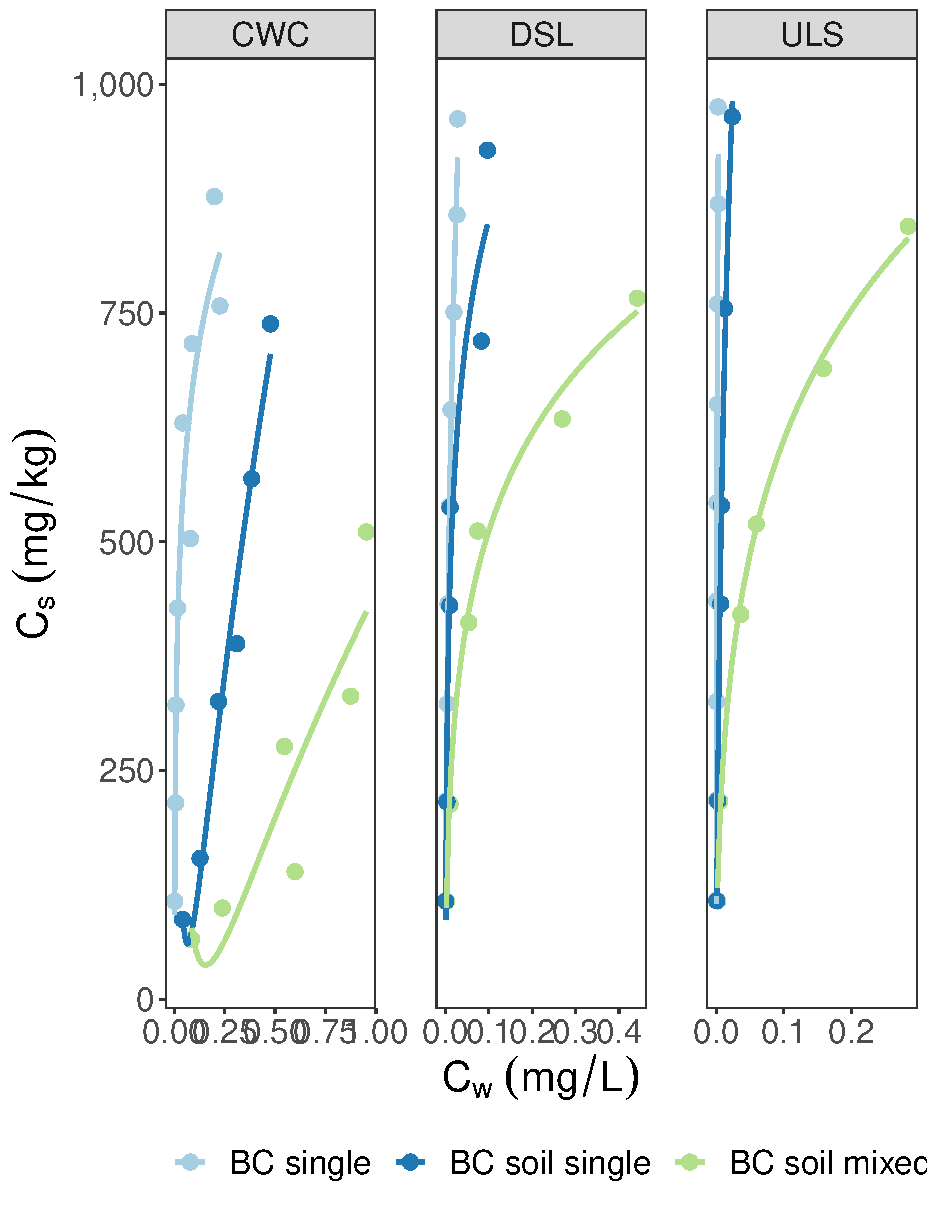
\includegraphics[width=0.8\textwidth]{R/figs/PFOA_linear.pdf}
    \caption{The differences in how much sorption of PFOA is attenuated in the BC single, BC mixed and BC soil mixed batch tests. Lines are fitted by a polylogarithmic function.}
    \label{fig:PFOA_nonlinear}
\end{figure}

\begin{figure}
    \centering
    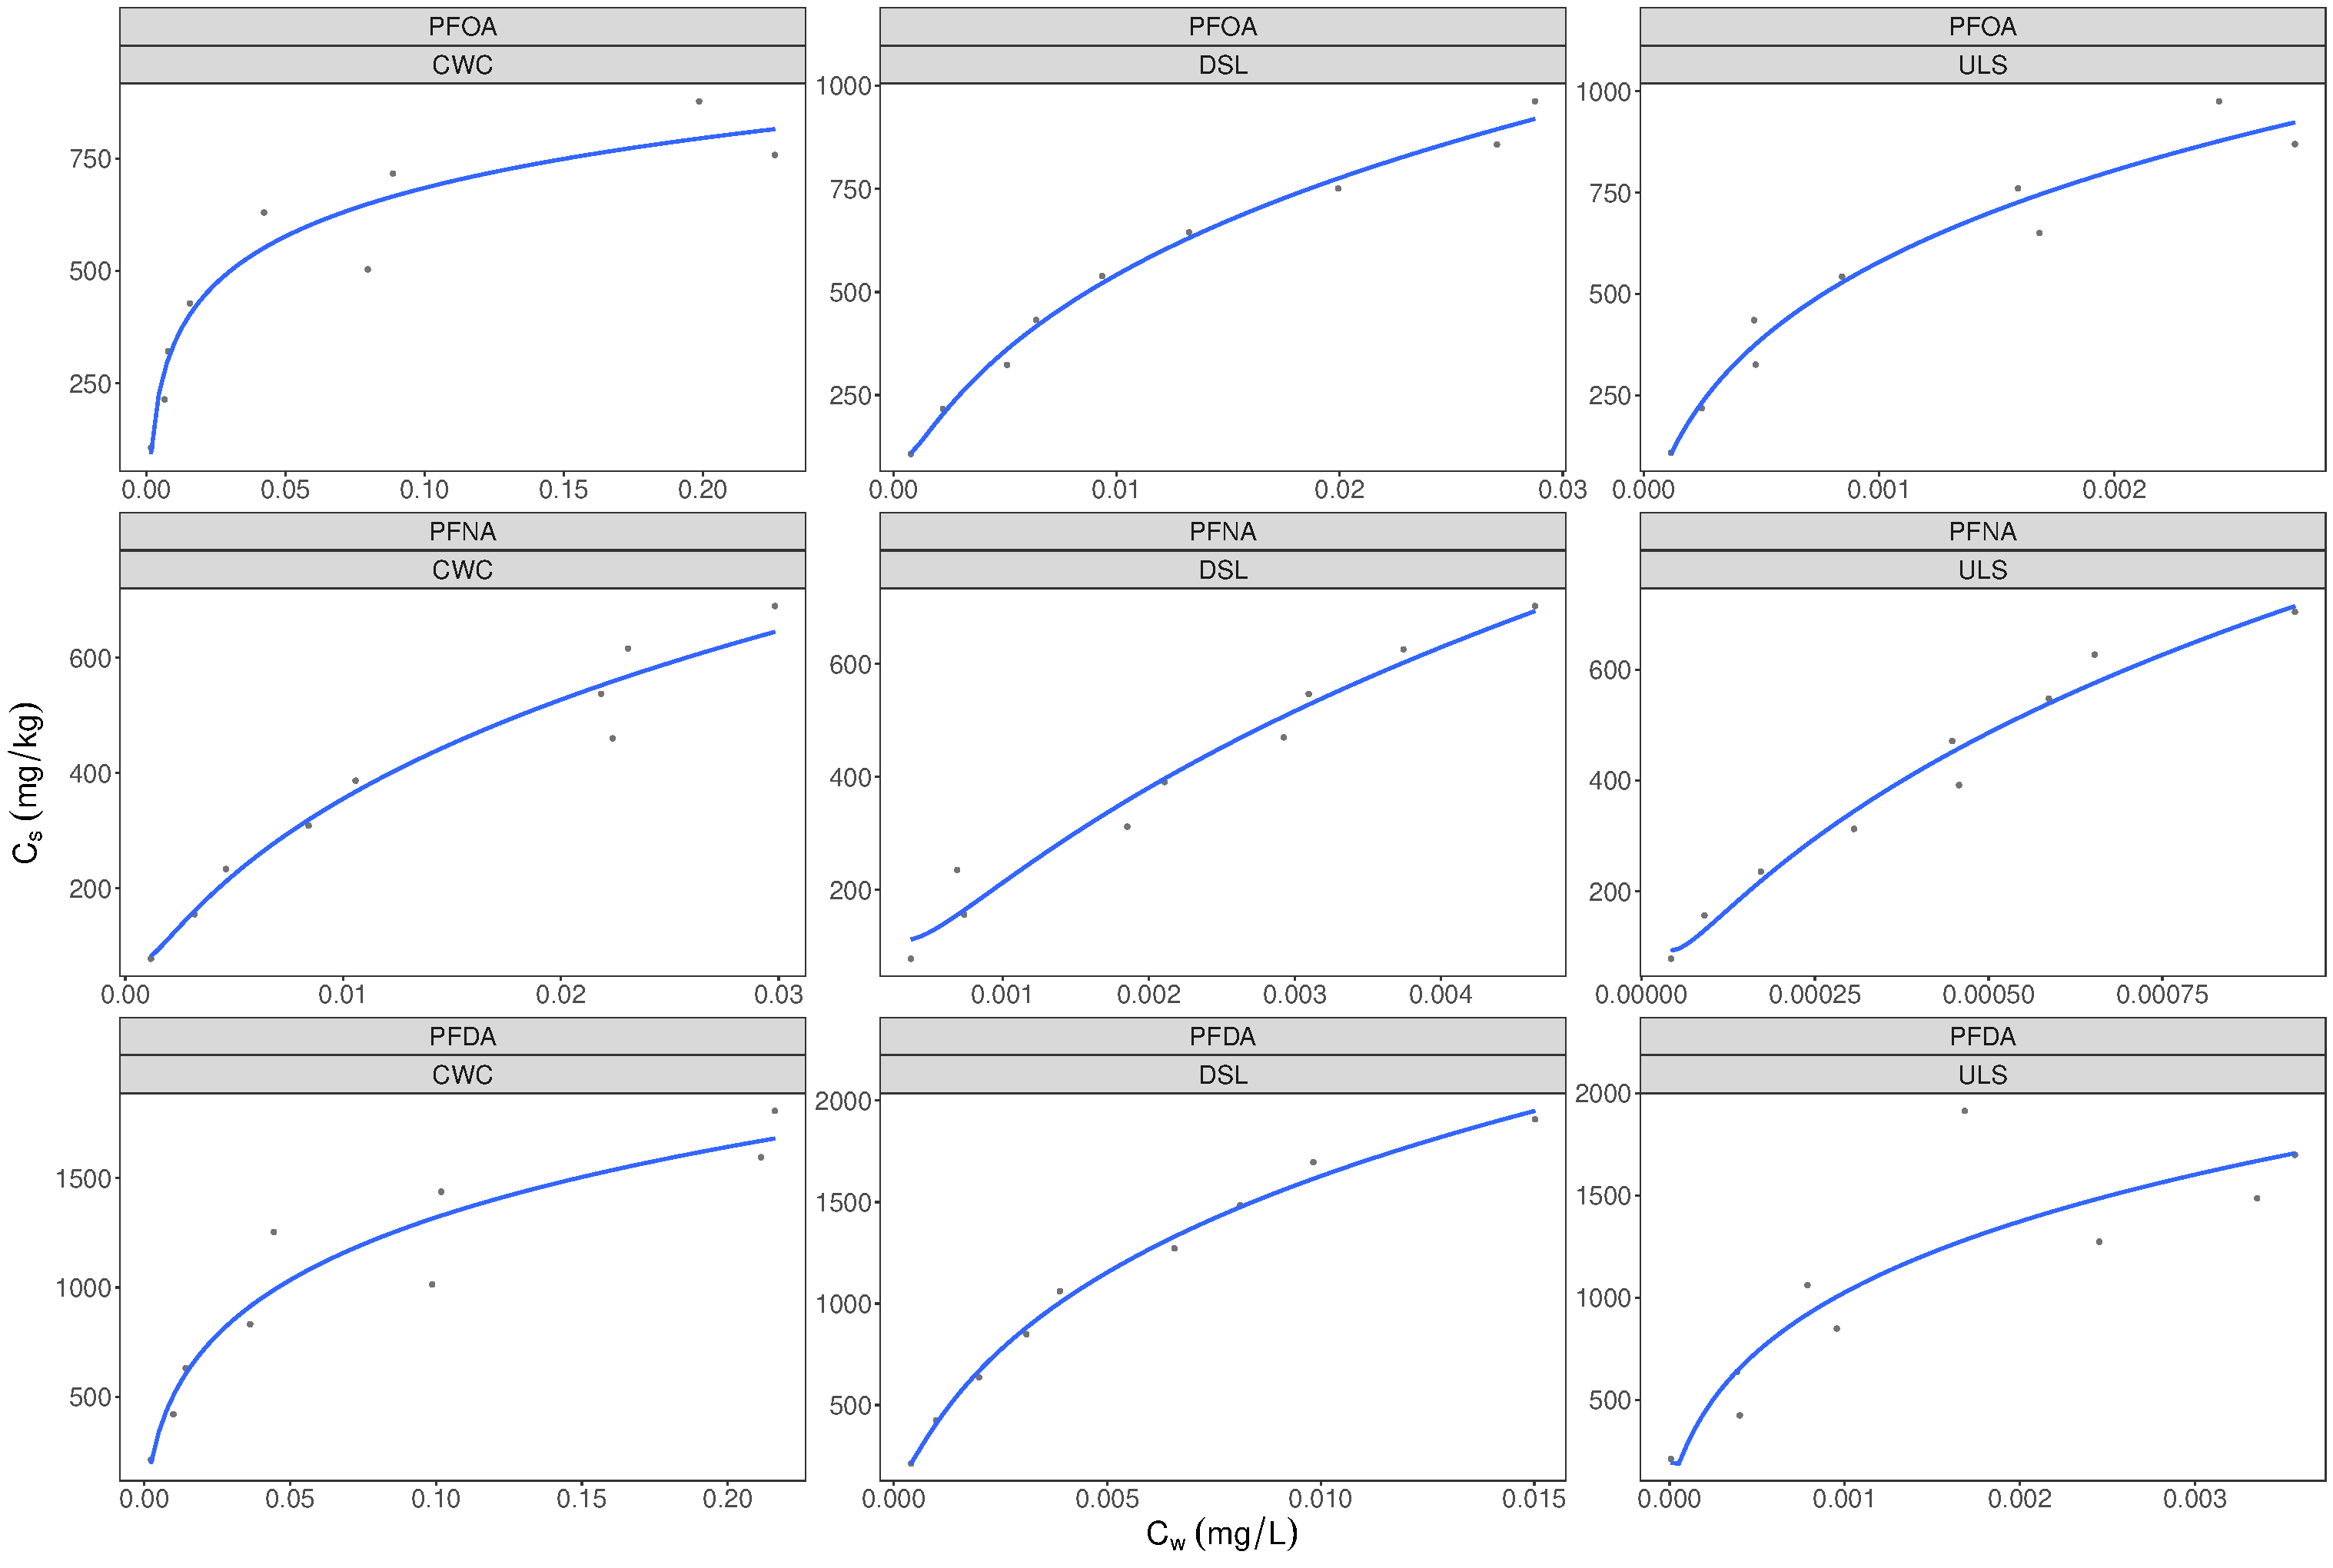
\includegraphics[width=\textwidth]{R/figs/BC_single_attenuation.pdf}
    \caption{Plots showing sorption attenuation by the presence of other PFCAs with increasing spiked concentrations. Lines are fitted by a polylogarithmic function.}
    \label{fig:nonlinear_OND} 
\end{figure}


%%%%%%%%%%%%%%%%%%%%%%%%%%%%%%%%%%%%%%%%%%%%%%%%%%%%%%%%%%%%%%%%%%%%%%%%%%%%%%%%%%%%%%%%%%%%%%%%%%%%%%%%%%%%%%%%%%%%%%%%%%%%%%%%%%%%%%%%%%%%%%%%%%%%%%%%%%%%%%%%%%%%%%%%%%%%%%%%%%%%%%%%%%%%%%%%%%%%%%%%%%%%%%%%%%%%%%%%%%%%%%%%%%%%%%%%%%%%%%%%%%%%%%%%%%%%%%%%%%%%%%%%%%%%%%%%%%%%%%%%%%%%%%%%%%%%%%%%%%%%%%%%%%%%%%%%%%%%%%%%%%%%%%%%%%%%%%%%%%%%%%%%%%%%%%%%%%%%%%%%%%%%%%%%%%%%%%%%%%%%%%%%%%%%%%%%%%%%%%%%%%%%%%%%%%%%%%%%%%%%%%%%%%%%%%%%%%%%%%%%%%%%%%%%%%%%%%%%%%%%%%%%%%%%%%%%%%%%%%%%%%%%%%%%%%%%%%%%%%%%%%%%%%%%%%%%%%%%%%%%%%%%%%%%%%%%%%%%%%%%%%%%

\section{Soil}\label{sec:Soil}
Before filtration of the batch tests with soil, each sample category (CWC-soil, DSL-soil, ULS-soil and soil only), despite being centrifuged, contained different degrees of suspended particles. This made it difficult to filter the samples that contained the most suspended particles. Filtration led to clogged filters that had to be changed up to three times per sample. The resulting filtrates varied in color \cref{fig:DOC}. These differences can be attributed to different amounts of dissolved organic carbon (\acrshort{DOC}). The sludge biochar-soil samples were more transparent than soil only and soil-CWC. The remarkable difference in DOC is attributed to DOC complexation with inorganic species present in the sludge chars, but not in CWC. Frequently clogged filters likely resulted in reduced filter pore size associated with the fact that some DOC was retained. This may have led to underestimating $C_w$, and thereby overestimating $K_d$ for soil which, in turn, became an issue when deriving $K_F$ for the biochar in these samples using \cref{eq:FreundLinSoil4}. Filter blanks were only prepared for BC-water samples that showed no significant effect (see \cref{apptab:FB}). Hence, the effect of reduced filter size by clogging cannot be quantified. In summary, the results and observations from the BC soil batch tests indicate that sewage sludge biochar binds DOC, and DOC in the filtrate is potentially responsible for an underestimation of $C_w$, and hence, overestimation of $K_{d,s}$. 

\begin{figure}
    \centering
    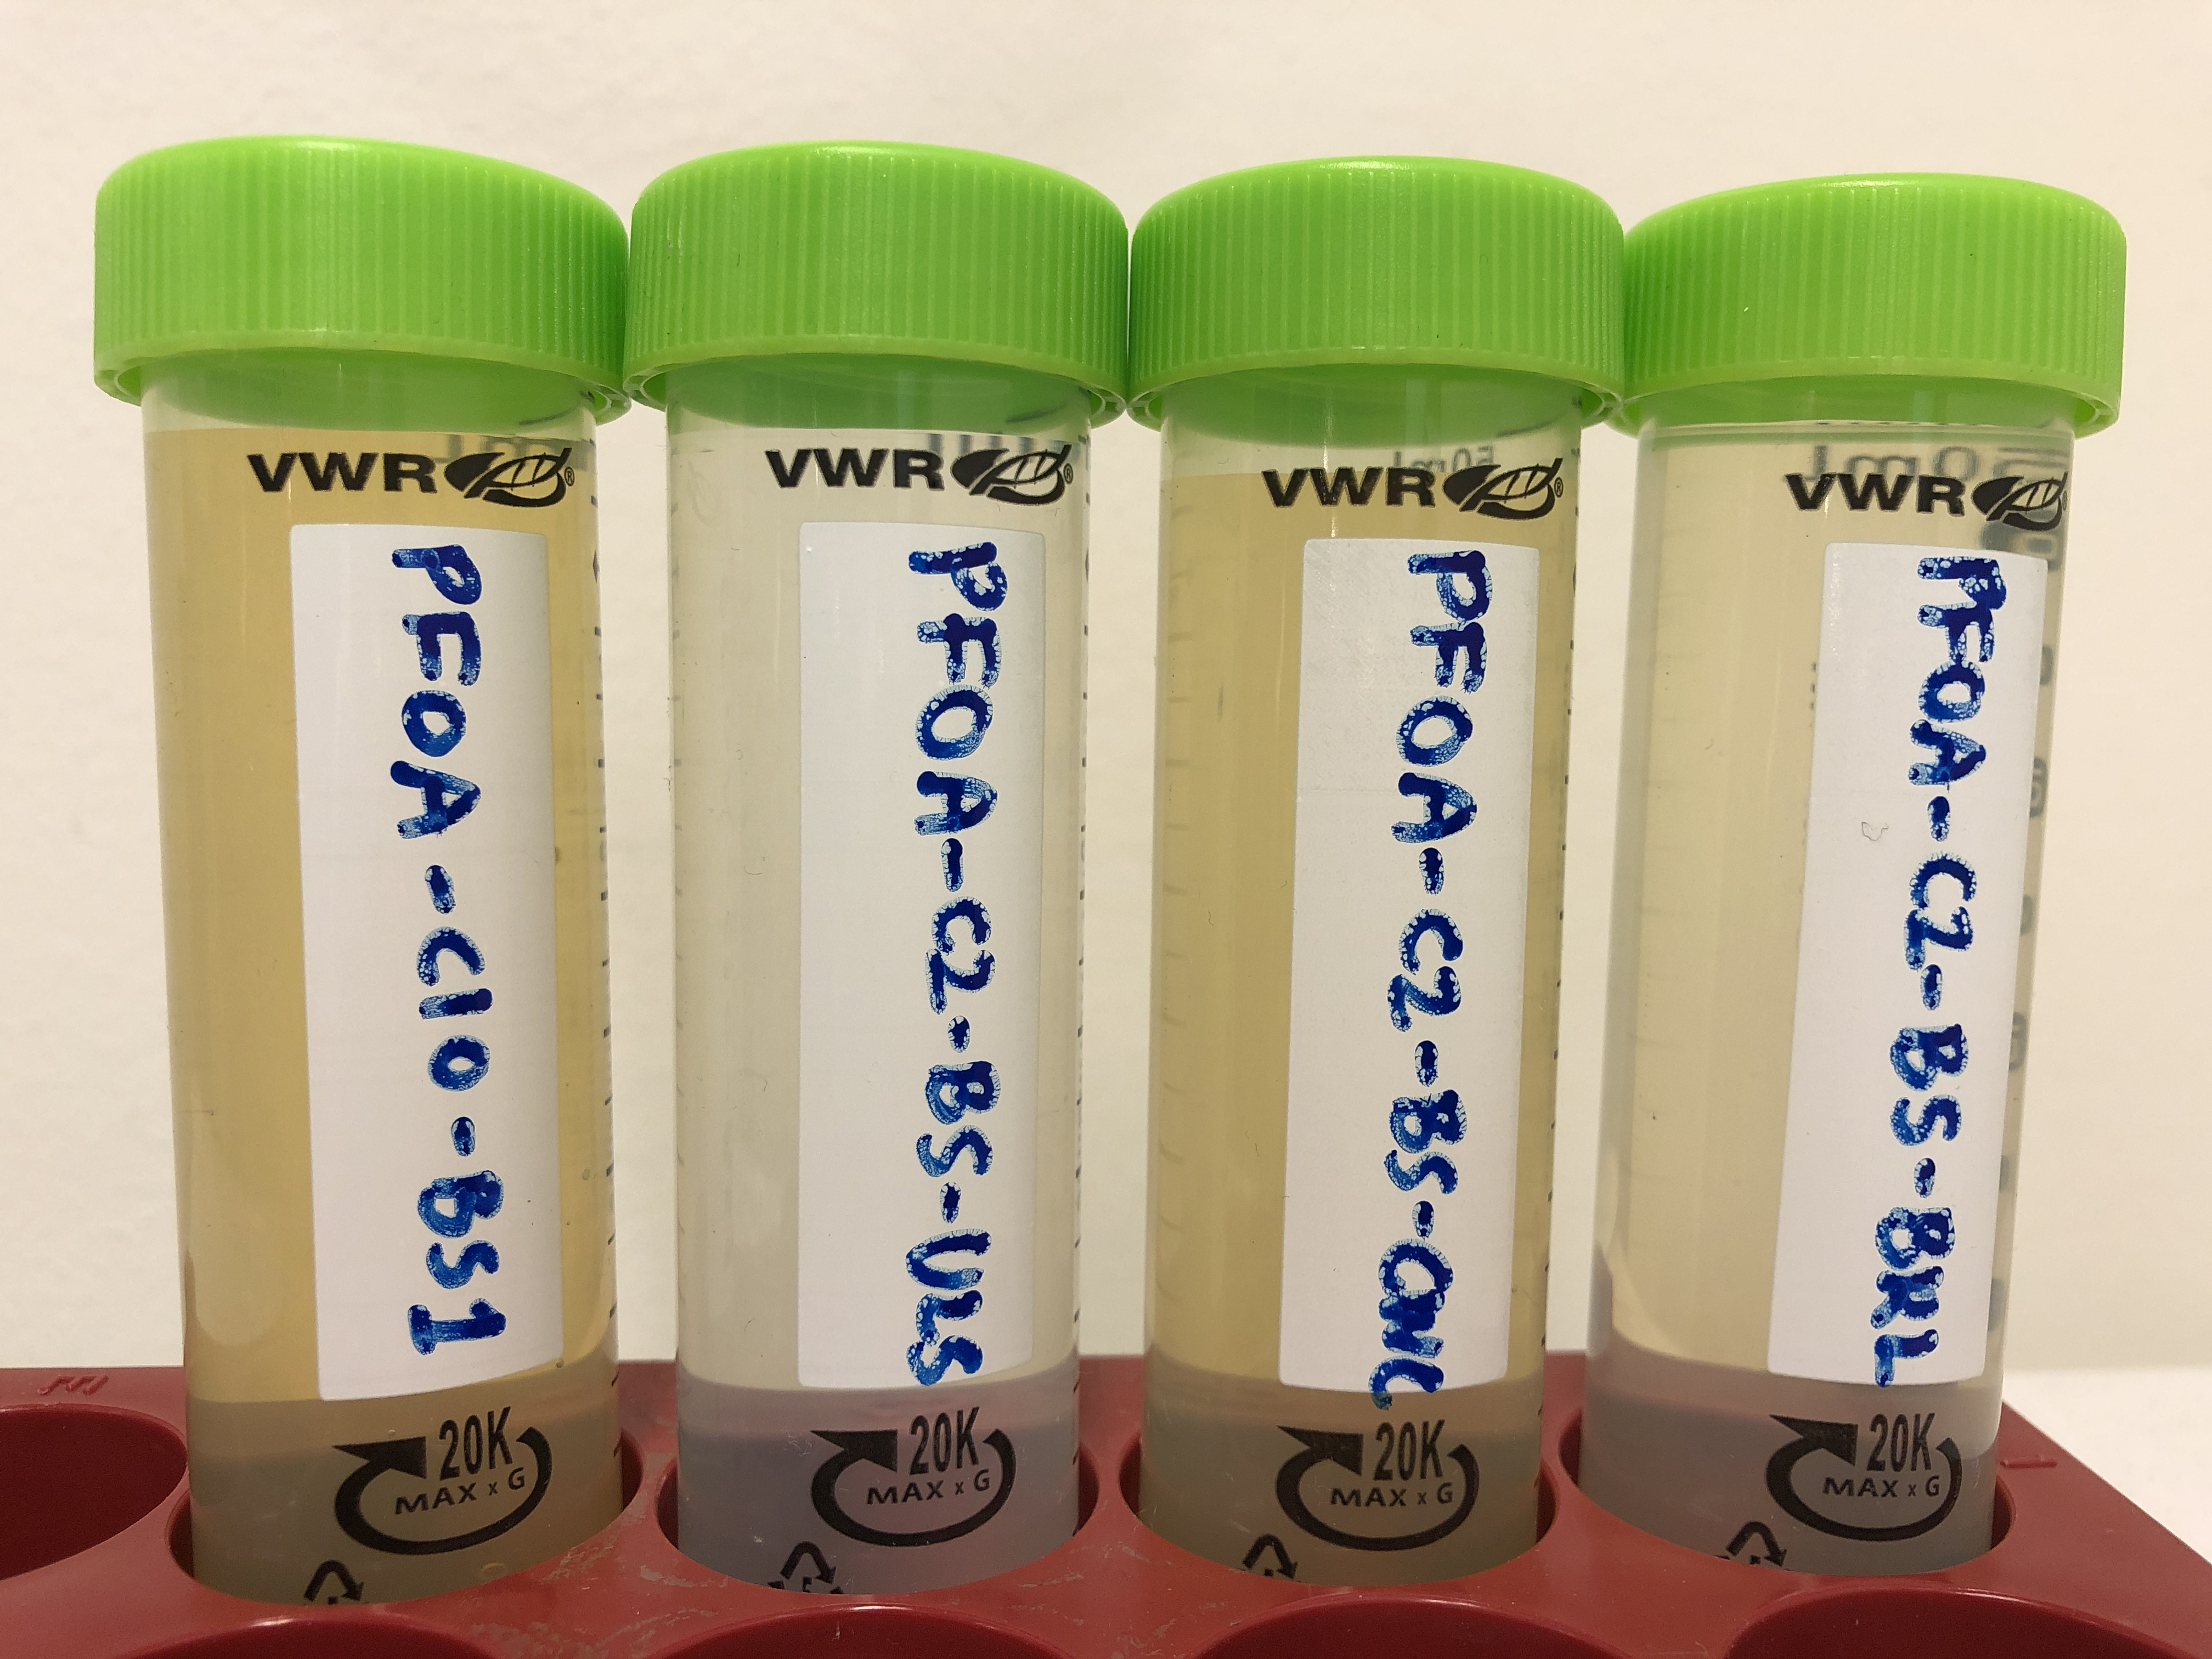
\includegraphics[width=0.7\textwidth]{Bilder/Samples/Filtrate_DOC.JPG}
    \caption{Color of filtrate for each biochar batch test. From left to right: soil only, soil+ULS, soil+CWC, and soil+DSL (BRL = DSL).}
    \label{fig:DOC}
\end{figure}

%%%%%%%%%%%%%%%%%%%%%%%%%%%%%%%%%%%%%%%%%%%%%%%%%%%%%%%%%%%%%%%%%%%%%%%%%%%%%%%%%%%%%%%%%%%%%%%%%%%%%%%%%%%%%%%%%%%%%
%%%%%%%%%%%%%%%%%%%%%%%%%%%%%%%%%%%%%%%%%%%%%%%%%%%%%%%%%%%%%%%%%%%%%%%%%%%%%%%%%%%%%%%%%%%%%%%%%%%%%%%%%%%%%%%%%%%%%
%%%%%%%%%%%%%%%%%%%%%%%%%%%%%%%%%%%%%%%%%%%%%%%%%%%%%%%%%%%%%%%%%%%%%%%%%%%%%%%%%%%%%%%%%%%%%%%%%%%%%%%%%%%%%%%%%%%%%

\subsection{Sustainable development goals (SDGs) \label{sec:SDGs}}
Several initiatives have been started related to the roles biochar can have in means to work towards reaching the United Nations Sustainable Development Goals (\acrshort{SDGs}) \citep{SDGs2015} and the European Green Deal of 2020. The European Green Deal of July 14, 2021 set that biochar is a means to achieve the goal to make Europe the first climate neutral continent through economic means: biochar is a potential commercial product in a circular economy\footnote{\url{https://ec.europa.eu/info/strategy/priorities-2019-2024/european-green-deal/delivering-european-green-deal_en}}. The 4 per mille initiative - Soils for food security and climate, was launched by France during the UN climate change conference of December 2015 (COP21)\footnote{\url{https://www.4p1000.org/}}. The 4 per 1000 mission is to increase soil carbon stocks in the first 30-40 cm of soil by 4 \textperthousand  annually to complement what is necessary efforts to compensate fossil GHG emissions globally. The goal is to scale biochar for global agricultural and remediation markets. If applied correctly, biochar can play an important role for carbon sequestration at the same time as serving as a soil amendment and fertilizer in agriculture. However, care must be taken because application of biochar in soil has shown to have a priming effect on soil native C by improving microbial populations, thereby increasing the decomposition rate of organic matter \citep{Ahmad2014}. However, in most cases, negative priming is seen (ref). The International Biochar Initiative (IBI) is a collaborative platform for science, industry, agriculture, government, and non-governmental organizations (EBC) to spread awareness about the benefits with biochar and develop biochar standards for safe and sustainable use\footnote{\url{https://biochar-international.org/about-ibi/}}. Norwegian initiatives related to the overarching project of this thesis (VOW\footnote{\url{https://www.ngi.no/eng/Projects/VOW-Valorization-of-Organic-Waste}}) include ZeroPM\footnote{\url{https://zeropm.eu}}, EarthResQe\footnote{\url{https://www.nmbu.no/en/services/centers/earthresque}}, SLUDGEEFFECT\footnote{\url{https://www.ngi.no/eng/Projects/SLUDGEFFECT}}, PERFORCE\footnote{\url{https://perforce3-itn.eu}}, among others set to contribute to achieve the European Green Deal. 

%%%%%%%%%%%%%%%%%%%%%%%%%%%%%%%%%%%%%%%%%%%%%%%%%%%%%%%%%%%%%%%%%%%%%%%%%%%%%%%%%%%%%%%%%%%%%%%%%%%%%%%%%%%%%%%%%%%%%%%%%%%%%%%%%%%%%%%%%%%%%%%%%%%%%%%%%%%%%%%%%%%%%%%%%%%%%%%%%%%%%%%%%%%%%%%%%%%%%%%%%%%%%%%%%%%%%%%%%%%%%%%%%%%%%%%%%%%%%%%%%%%%%%%%%%%%%%%%%%%%%%%%%%%%%%%%%%%%%%%%%%%%%%%%%%%%%%%%%%%%%%%%%%%%%%%%%%%%%%%%%%%%%%%%%%%%%%%%%%%%%%%%%%%%%%%%%%%%%%%%
